%Plantilla Memoria T�cnica:
%Modificada por: Brenda Mariana Casillas Gonz�lez
%Última Modificación: 02-01-2023

%------------------------------CONFIGURACION DEL DOCUMENTO

\documentclass[12pt,letterpaper,spanish, xcolor=table]{report}
\usepackage[centertags]{amsmath}
\usepackage{amsfonts}
\usepackage{amssymb}	
\usepackage[utf8]{inputenc} % Usa solo esta línea
\usepackage{amsthm}
\usepackage[T1]{fontenc}
\usepackage{epsfig}
\usepackage{booktabs}
\usepackage{graphics}
\usepackage{amsmath}
\renewcommand{\baselinestretch}{1.5}
\renewcommand{\thefigure}{\thesection.\arabic{figure}}
\numberwithin{figure}{subsection}
\makeatletter
\@addtoreset{figure}{section}
\makeatother
\usepackage[spanish,activeacute]{babel}
\usepackage[numbers]{natbib}
\usepackage[hyphens]{url}
\usepackage{enumerate}
\usepackage{float}

\newenvironment{dedication}{\newpage\large\null\em\vskip1in}%
{\vfill}

\topmargin -1 in \oddsidemargin 0in \evensidemargin 0in
\textwidth 6.5in
\textheight 9in \pagestyle{myheadings}

% -----------------------------------INICIO DEL DOCUMENTO ---------------------------------------------------------------

\begin{document}
	
% Para la elaboraci�n de esta memoria t�cnica se debe usar un editor profesional que soporte Latex, como recomendaci�n se puede usar el WinEdt.

% El resultado que se sube a la plataforma debe ser en formato PDF

% Es importante mencionar que la redacci�n de este documento se debe hacer en tercera persona, cuidando escrupulosamente la ortograf�a, redacci�n y contenido, evitando el uso y abuso de adjetivos.
	
% ----------------------------------- CONTRAPORTADA -------------------------------------------------------------------------

%Se deben modificar los datos de la empresa, proyecto, asesores y alumnos
	
\thispagestyle{empty}

\begin{table}[ht]
  \centering
	\begin{tabular}{rr}
		\begin{minipage}[b]{0.05\linewidth}
		\hbox{
\psfig{file=Imagenes/logoUTZMG.jpg,height=1in,width=.8in}}
		\end{minipage}
	&
	\begin{minipage}[b]{.9\linewidth}
		\begin{center}
			\large{UNIVERSIDAD TECNOLÓGICA \\ DE LA ZONA METROPOLITANA DE GUADALAJARA}\\
		\end{center}
	\end{minipage}
	
	\end{tabular}%
\end{table}%

\begin{center}
	
\large{\textbf{MEMORIA TÉCNICA REALIZADA EN:}}
 \\ PiSA Farmacéutica

%%Logo de la empresa
\centerline{\hbox{
\psfig{file=Imagenes/logoPISA.png,height=1.2in,width=3in}}}

\large{\textbf{PROYECTO:} Soluciones Informáticas para Unidades de Servicios Administrativos}

\vspace{0.1in}
\large{\textbf{PARA OBTENER EL GRADO DE:}}

\large{Ingeniería (ING) en:}
\vspace{0.05in}

\large{DESARROLLO Y GESTIÓN DE SOFTWARE}
\\
\large{PRESENTADO POR:}

Jessica Aguilar Valderrama %(Empezando con el nombre  y después apellidos)

Luis Manuel Gómez López %(Empezando con el nombre  y después apellidos)

\vspace{0.2in}

\begin{tabular}{cc}
	\vspace{0.2in}
	\textbf{ASESOR INDUSTRIAL} & \textbf{ASESOR ACADÉMICO} \\
	
	Ricardo Adolfo González Pineda & Mildred Green Gama\\
	\multicolumn{2}{c}{\textbf{COORDINADOR DE CARRERA}
	\vspace{0.2in}
	} \\
	
	\multicolumn{2}{c}{
			Lizbeth Noriega Gutiérrez }
	\end{tabular}
	
\end{center}
%\vspace{0.1in}
\begin{flushright}\small{ TLAJOMULCO DE ZUÑIGA, JALISCO, ABRIL DEL 2025} \end{flushright}

\newpage



% ------------------------------ PORTADA -----------------------------------------------------

%Se deben modificar los datos de la empresa, proyecto y alumnos



\thispagestyle{empty}


\begin{center}
	
 \begin{minipage}[b]{.9\linewidth}
	\begin{center}
		\vspace{0.2in}
		\large{UNIVERSIDAD TECNOLÓGICA DE LA ZONA \\METROPOLITANA DE GUADALAJARA}\\
		\large{DIRECCIÓN DE DESARROLLO Y GESTIÓN DE SOFTWARE}\\
	\end{center}
\end{minipage}
\vspace{0.3in}



\centerline{\hbox{
\psfig{file=Imagenes/utzmg.png,height=2.2in,width=1.7in}}}

\LARGE{\textbf{\textsc{ Soluciones Informáticas para Unidades de Servicios Administrativos}} }

\vspace{0.3in}
\large{\textbf{MEMORIA TÉCNICA REALIZADA EN:}}
 \\ \textsc{PiSA Farmacéutica}
		
\vspace{0.2in}
\large{\textbf{PARA OBTENER EL GRADO DE:}}

\large{Ingeniería (ING) en:}

\large{DESARROLLO Y GESTIÓN DE SOFTWARE}
\\

\vspace{0.2in}
\large{PRESENTADO POR:}


\textsc{} Jessica Aguilar Valderrama %(Empezando con el nombre y despu�s apellidos)

\textsc{} Luis Manuel Gómez López

\vspace{0.3in}
\small{ ABRIL 2025}
\end{center}
%\vspace{0.1in}


\newpage


% -------------------------------------- DEDICATORIA ---------------------
% Esta secci�n es opcional, pero se recomienda que se ponga, se puede redactar hasta el final y tratar que no sea mayor a una cuartilla.

		\thispagestyle{empty}
		\addcontentsline{toc}{chapter}{Agradecimientos}
		
		\begin{dedication}
			Jessica Aguilar Valderrama:
			
			Hoy quiero expresar mi más grande agradecimiento a todas las personas que contribuyeron a concluir mi formación académica y claro, en la realización de esta tesina. En primer lugar, quiero agradecer a la Mtra. Mildred por su orientación en este proceso, por el apoyo que me brindó, más que lo académico le agradezco por entender en cada momento mi situación con mi vida laboral, a pesar de siempre estar preocupada por esto, sabía que iba a obtener una respuesta amigable de su parte, por esto y más, gracias. De igual manera quiero hacer mención a las colaboradoras de mi trabajo, las cuales me acompañaron en esta difícil travesía, mi querida Yaredhit, te agradezco desde el fondo de mi corazón cada día, hora y momento en el que sin importar las circunstancias, jamás me dejaste sola con todo este peso, gracias por tu apoyo incondicional que en mis peores momentos nunca me sentí sola, te quiero.\\
			
			Gracias a mi Madre y Hermana mayor, las cuales me han ayudado a formarme como una persona, con sus tropiezos pero ante todo nunca me han dejado de querer, al igual que yo a ustedes, sepan que este logro es también de ustedes, gracias Madre, por ser mi Madre, gracias por darme tantas oportunidades que tal vez tú no tuviste, gracias por enseñarme lo bonita y buena persona que puede ser alguien, gracias por escucharme y aconsejarme, no me alcanzaría la hoja ni una tesis completa para agradecerte todo lo que has hecho por nosotros. A mi hermana, le agradezco por guiarme, hacerme sentir capaz cada que siento que el mundo me pisotea, gracias por ponerme la vara tan alta como decían mis papás , eres un ejemplo MI ejemplo de la mujer que me quiero convertir , eres mi ser de luz y mi persona favorita aunque no te lo digo siempre.\\
			
			A mi padre, no hay palabras para agradecerte lo mucho que has hecho por mi, lo que me has enseñado a lo largo de mi vida, gracias por exigirme, enseñarme que hay que tener resiliencia, gracias por ser mi mejor amigo , porque gracias a ti sé lo que es que alguien me espere en casa después de mi rutina, por ti siempre he querido ser más , formarme como persona, y una persona de la cual estés orgulloso, un te amo se queda corto, pero si, te amo pulguitas, no pude tener un mejor compañero en la vida, gracias.\\
			
			A mis amigos , Manuel y Toño, no quiero pasar desapercibido el vínculo mas valioso que obtuve al estar con ustedes como compañera de carrera, gracias por su amistad incondicional a lo largo de esta travesía , gracias por nunca haberme hecho sentir que cada emoción obtenida era inválida, ustedes más que nadie saben lo que significa haber llegado hasta aquí , y sobretodo llegar aquí juntos, gracias por todas las veces que me sostuvieron , gracias porque también ustedes no se rindieron en el camino , sepan que son personas valiosas e inteligentes con las cuales fuí muy feliz y por las cuales disfruté esta travesía , me gusta pensar que cuando perdí a mis mejores amigos fue porque sabían que me dejaban con ustedes, rodeada de cariño y de una amistad inquebrantable, les quiero y deseo que toda su vida esté rodeada de éxitos y tranquilidad, gracias por llegar al final del camino conmigo, gracias por ser mis amigos, de esos que se cuentan con los dedos.\\
			
			Por último quiero agradecerle a mi pareja , Pepe , una persona que me acompañó desde el día uno en esta travesía, el mismo que se convertiría en mi mayor confidente, gracias por permitirme conocerte, como amiga y como pareja, siempre me ha tocado el corazón ver como tú ves la vida aún en su etapa más compleja, gracias por entenderme cuando ni yo lo hago, ambos sabemos lo que pasamos para llegar hasta aquí y más llegar juntos, deseo que esto sea solo el principio de muchos logros juntos, gracias por llenarme de un amor que ni siquiera sabía que necesitaba, gracias por aceptarme un taxi, te amo.\\
			
			En fin, fue un largo camino pero de la mano de estas personas lo repetiría sin pensarlo, gracias.
		\end{dedication}

		\begin{dedication}
			
			Luis Manuel Gómez López:
			
		Fue un camino largo, un camino de sacrificios, desveladas, buenos y malos momentos. Apesar de todo, siempre tuve con quién contar.\\
		
		Me gustaría comenzar agradeciendo a uno de los pilares más fundamentales de mi vida, mis padres. No hay palabras u obsequios que representen lo agradecido que estoy con ustedes, doy gracias a Dios por darme unos padres que me han demostrado que con ayuda todo se puede resolver, que no existe lo imposible. Es simplemente decir gracias, pero detrás de una simple palabra conlleva el reconocimiento del esfuerzo y sacrificio que han hecho por mí. Espero que algún día la vida recompense todas mis acciones y poder cumplir lo que en algún momento les prometí. A mis hermanos que siempre se han encargado hacer momentos únicos para llevarlos en el corazón, dónde se han compartido risas y corajes, sabiendo que el fondo siempre podré contra con ustedes en cualquier situación agradeciendo su apoyo en cada sueño o meta.\\
		
		Sin dejar a un lado también debo reconocer el apoyo incondicional que me han brindado mis abuelitos, que siempre se han preocupado por mi bienestar y nunca han dudado en ayudarme en cualquier situación, agradezco cada consejo que tengan por seguro que siempre van estar en mi corazón.\\
		
		A mi tío Marcelo, le agradezco el tiempo que se tomó de sus días tan ocupados para reparar mi equipo de trabajo y del hecho de nunca quejarse o hacer las cosas para recibir algo a cambio estaré agradecido toda la vida.\\
		
		Aunque no fueron parte de la universidad, me gustaría mencionar a mis amistades de la infancia. Emmanuel y Christopher espero que nunca acaben nuestras aventuras y momentos inolvidables, ustedes son parte fundamental en mi vida.\\
		
		Apesar de no estar presente debo agradecer a esa amistad que sin importar la distancia nunca fue una excusa para estar presente cada día, luego nos veremos para hablar de lo maravilloso que es la vida.\\ 
		
		A mí grupo de universidad, mis compañeros, más bien dicho mis amigos. Fueron una parte fundamental para que mi estancia en la universidad fuera única, con momentos que nunca olvidaré. Me hicieron sentir que como en familia, aprender de cada uno de ustedes fue una gran experiencia. Creo que les debo mucho de lo poco que les he agradecido por siempre hacerme reír, de estar en momentos difíciles y nunca dejarme abajo.\\
		
		Toño, Pepe, Alexis, Angiie, Mombe, Anthony, Edgar, Thalía, Luis, Brian, Diana, Braulio, Carlos. Cómo mucho amor se los agradezco.\\
		
		A mí compañera de estadías, mi más real, mi mejor amiga, Jessica. No cabe duda que se convirtió en una amistad única y especial.  Son muchas cosas por las cuál debo agradecerte por todo lo que has hecho por mi y la confianza que me has dado para cada situación, no hay nada en el mundo que pueda expresar ese sentimiento y un gracias se queda muy corto. Estoy seguro que Dios, la vida o el destino va a cumplir cada uno de tus sueños y espero estar ahí para recordarte que te los mereces. Gracias por existir.\\
			
		\end{dedication}

%-------------------------------- �NDICE


\tableofcontents


% --------------------------------------- CAP�TULOS DEL DOCUMENTO ----------------------------------------
% ____________________________________________________________________________________


\pagenumbering{arabic}
\oddsidemargin 0.2in \textwidth 6.5in \topmargin -0.25in
\textheight 9in \pagestyle{myheadings}
	
	
\newpage

% CAPITULO INTRODUCCI�N. Enmarca y situa el trabajo a realizar. Tiene por objeto proporcionar una visi�n general del documento.
%____________________________________________________________________________________________________________________


\chapter{Introducción}
\newpage

La presente Memoria Técnica documenta el trabajo realizado en diversos proyectos internos de PiSA, consolidando la evidencia de las actividades, análisis y entregables generados en cada iniciativa. Su propósito es registrar de manera estructurada y detallada cada una de las fases involucradas en los proyectos en los que se ha participado, asegurando la trazabilidad y el respaldo de la información técnica y funcional que los conforma.\\

Se detallan los procesos llevados a cabo, desde el levantamiento de requerimientos hasta la definición de épicas y criterios de aceptación, así como el diseño de casos de prueba. Cada una de estas secciones refleja el enfoque metodológico aplicado en cada proyecto, proporcionando un panorama integral sobre las especificaciones técnicas, validaciones y consideraciones que han guiado el desarrollo de las soluciones implementadas.\\

Resaltando la importancia de una documentación bien estructurada en el éxito de cada iniciativa. Se evidencia el impacto positivo de un enfoque meticuloso en la planificación y documentación del desarrollo de software, asegurando entregables de alto valor y alineados con las necesidades de la organización.\\




% CAPITULO ANTECEDENTES Y DESCIPCI�N DE LA EMPRESA. Tiene por objeto proporcionar una visi�n general del documento.
%____________________________________________________________________________________________________________________
\chapter{Antecedentes y Descripción de la Empresa}
\newpage


%Nota: Los puntos que siguen son una propuesta, pongan solo los puntos que apliquen en su empresa y que los permitan poner, tambi�n puede agregar otros puntos si lo cree conveniente.

\section{Ubicación}
	
\begin{figure}[htp]
	\centering
	Av España 1802, Moderna, 44190 Guadalajara, Jal.
	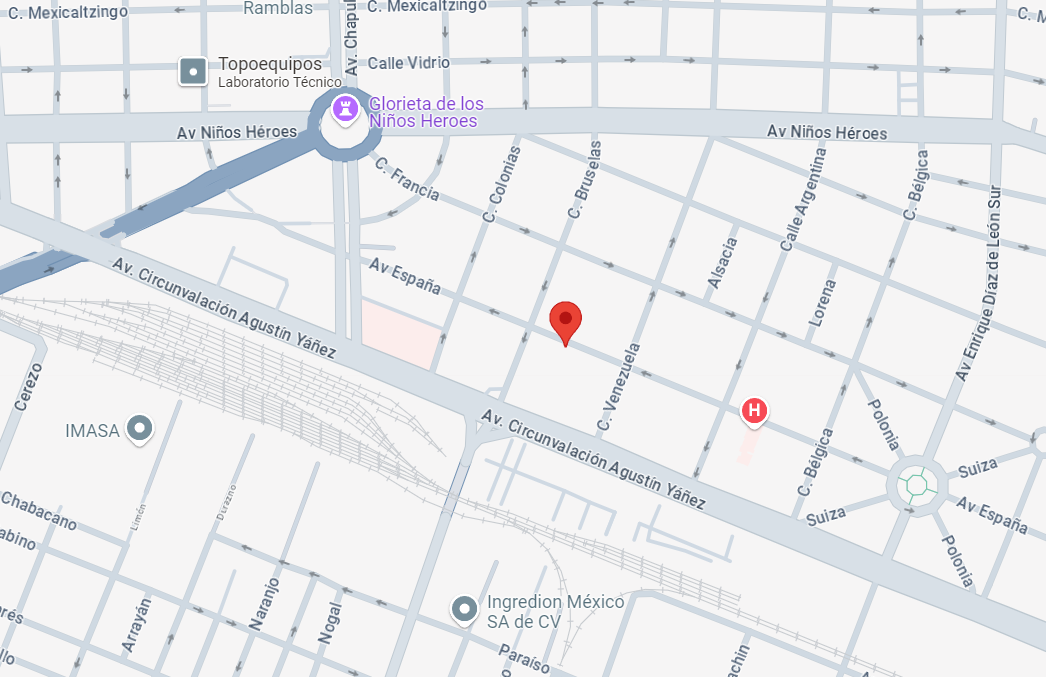
\includegraphics[width=0.8\textwidth]{Imagenes/ubicacion.png}
	\caption{Mapa ubicación Laboratorios PiSA S.A DE C.V}\label{a1}
\end{figure}


% Poner la direcci�n y un mapa que puede salir de maps.google.com


\section{Misión}
Somos un Grupo de Empresas Responsables, confiables, éticas, con vocación de servicio; comprometidas con sus colaboradores y la salud.

\section{Visión}
Permanencia a través de innovación y crecimiento acelerado en México y en el extranjero.
	
\section{Organigrama}

\begin{figure}[H]
	\centering
	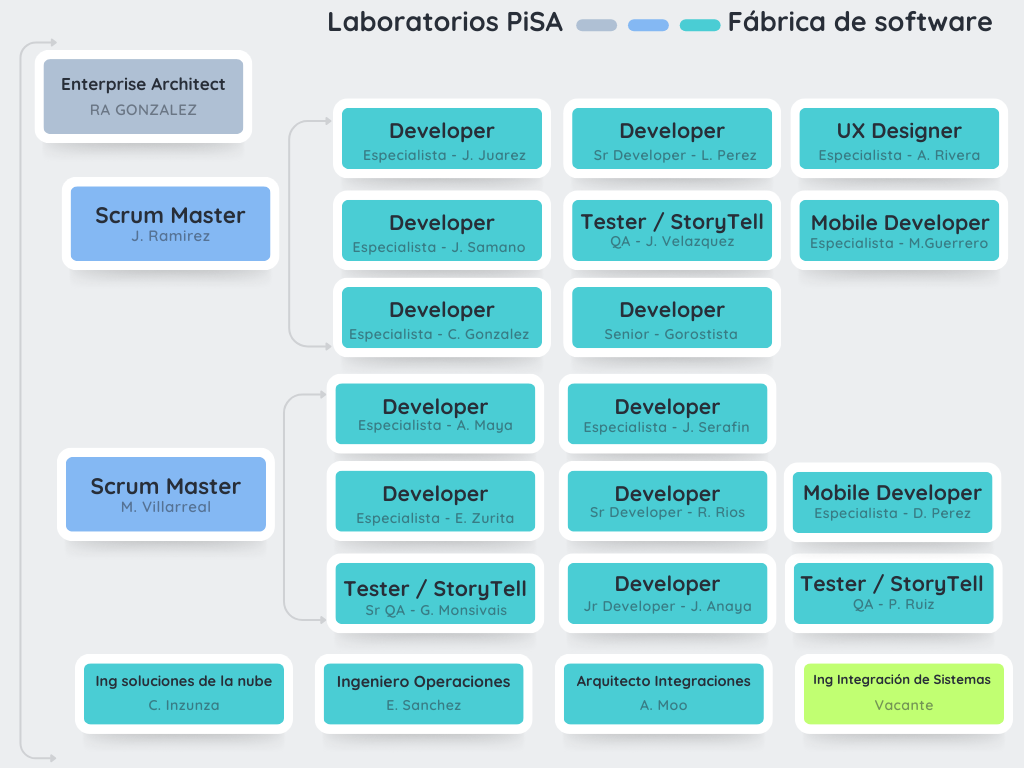
\includegraphics[width=0.9\textwidth]{Imagenes/OrganigramaPisa.png}
	\caption{Organigrama de Fábrica de Software}\label{a1}
\end{figure}
	
\section{Giro de la empresa}

PiSA Farmacéutica es una empresa dedicada a la fabricación, comercialización y distribución de medicamentos y dispositivos médicos en el tratamiento de un amplio ramo de la salud

\section{Historia}

Pisa Farmacéutica es una empresa mexicana del sector farmacéutico que tuvo su origen en 1945, fundada por el Profesor Don Miguel Álvarez Ochoa. Con la colaboración de destacados profesionales de la salud, estableció Productos Infantiles S.A. en respuesta a la necesidad de la época: desarrollar medicamentos especialmente diseñados y formulados para la población infantil.\\

En sus inicios, Productos Infantiles S.A. produjo más de diez medicamentos dirigidos principalmente a niños, entre ellos: INFRAFEN, gotas para tratar los cólicos en bebés; INFALGINA, gotas analgésicas y antipiréticas; y INFANEUMIL, jarabe para la tos, los cuales fueron ampliamente aceptados.\\

El Profesor Álvarez Ochoa supervisaba personalmente cada etapa del proceso, desde la adquisición de materias primas y materiales hasta la fabricación, distribución, promoción y venta de los productos. Gracias a su formación académica y experiencia en la industria farmacéutica mexicana, estableció la calidad como la principal y más estricta condición en la elaboración de los medicamentos, asumiendo esta responsabilidad de manera directa.\\

El esfuerzo, el trabajo y el conocimiento de quienes integraban la empresa en aquella época se reflejaron en su crecimiento. Este desarrollo sostenido llevó a una transformación significativa, y diez años después, Productos Infantiles S.A. evolucionó para convertirse en Laboratorios Pisa S.A. de C.V.\\

Actualmente, tras más de 70 años de trayectoria y con más de 25,000 colaboradores, Pisa Farmacéutica se ha consolidado como la empresa farmacéutica mexicana líder en el sector. Su prestigio y la confianza de médicos, enfermeras, instituciones y pacientes respaldan su compromiso con la elaboración de productos de la más alta calidad. Además, la empresa cumple con todas las normas nacionales e internacionales que regulan la producción farmacéutica, manteniendo un enfoque constante en la innovación, la mejora continua y el crecimiento.\\



\newpage
% -------------------------------- CAPITULO PROBLEM�TICA --------------------------------------
%____________________________________________________________________________________________________________________
	
\chapter{Problemática y Descripción del Proyecto}
\newpage

% En esta secci�n se deber� redactar un planteamiento de la problem�tica que se pretende resolver.
\section{Problemática}

	En el desarrollo de software, una administración de proyectos eficiente es clave para garantizar calidad y cumplimiento de objetivos. Sin embargo, la falta de documentación técnica bien estructurada dificulta la comprensión del proyecto y afecta el trabajo de equipo, provocando así que la documentación sea inconsistente, incompleta o desactualizada, lo que dificulta la aplicación de pruebas precisas y la identificación temprana de errores.  \\
	
	En la historia de PiSA, en algunos sistemas no normativos, la ausencia de una documentación clara y bien definida genera problemas en la comunicación entre los diferentes equipos de trabajo, dificultando la alineación de objetivos y la comprensión de los requerimientos del sistema. Esto impacta negativamente en la calidad del producto final, ya que se incrementan los riesgos de malinterpretaciones, modificaciones no documentadas y errores en la implementación.
	

%Escribir un resumen de su proyecto en donde se hable del aspecto económico, operativo, técnico, humano, objetivos, etc.
\section{Descripción del Proyecto}
	
	Desarrollar un enfoque estructurado para la elaboración de documentación técnica en proyectos de software, asegurando que sirva como una herramienta clave para la administración eficiente del desarrollo y control de calidad. Esta documentación permitirá mejorar la comunicación entre los equipos, optimizar la gestión de requisitos y garantizar que el software cumpla con los estándares y las expectativas del usuario final.


%Describir cual es el objetivo general que persigue el proyecto.
\subsection{Objetivo General}

	Se enfocará en la creación de guías, plantillas y metodologías que permitan documentar de manera clara los requerimientos, la arquitectura y los criterios de aceptación del software. Se trabajará en conjunto con el equipo de Quality Assurance (QA) para garantizar que la documentación cumpla con los estándares de calidad necesarios para la ejecución eficiente de pruebas y validaciones. Reduciendo el riesgo de errores y mejorando la trazabilidad del proyecto. Con ello, se busca optimizar la administración del proyecto, reducir tiempos de desarrollo y asegurar que el producto final cumpla con las expectativas del usuario y los estándares de la industria.\\
	
	Esta documentación facilitará la comprensión del sistema, mejorará la comunicación entre equipos y permitirá una mejor gestión de cambios, optimizando el proceso de desarrollo.
	


%Describir cuales son los objetivos específicos que persigue el proyecto. Mínimo deben ser dos y estos deben abonar al objetivo general
\subsection{Objetivos Específicos}

	1. Establecer lineamientos para la estructuración de documentos que faciliten la gestión de requisitos y planificación del desarrollo.\\
	
	2. Mejorar la comunicación entre los equipos de trabajo mediante documentación clara y organizada.\\
	
	3. Reducir el riesgo de errores en el desarrollo a través de documentación detallada y bien estructurada.\\
	
	4. Garantizar que la documentación técnica cumpla con estándares de calidad y facilite la trazabilidad del proyecto.\\
	
	5. Apoyar al equipo de Quality Assurance (QA) en la elaboración de documentación que permita validar el cumplimiento de los requisitos del software.\\

	
	
%Describir de manera detallada las actividades para el desarrollo de la estadía y/o proyecto (Diagrama de Gantt).
\subsection{Planeación}

	\begin{figure}[H]
		\centering
		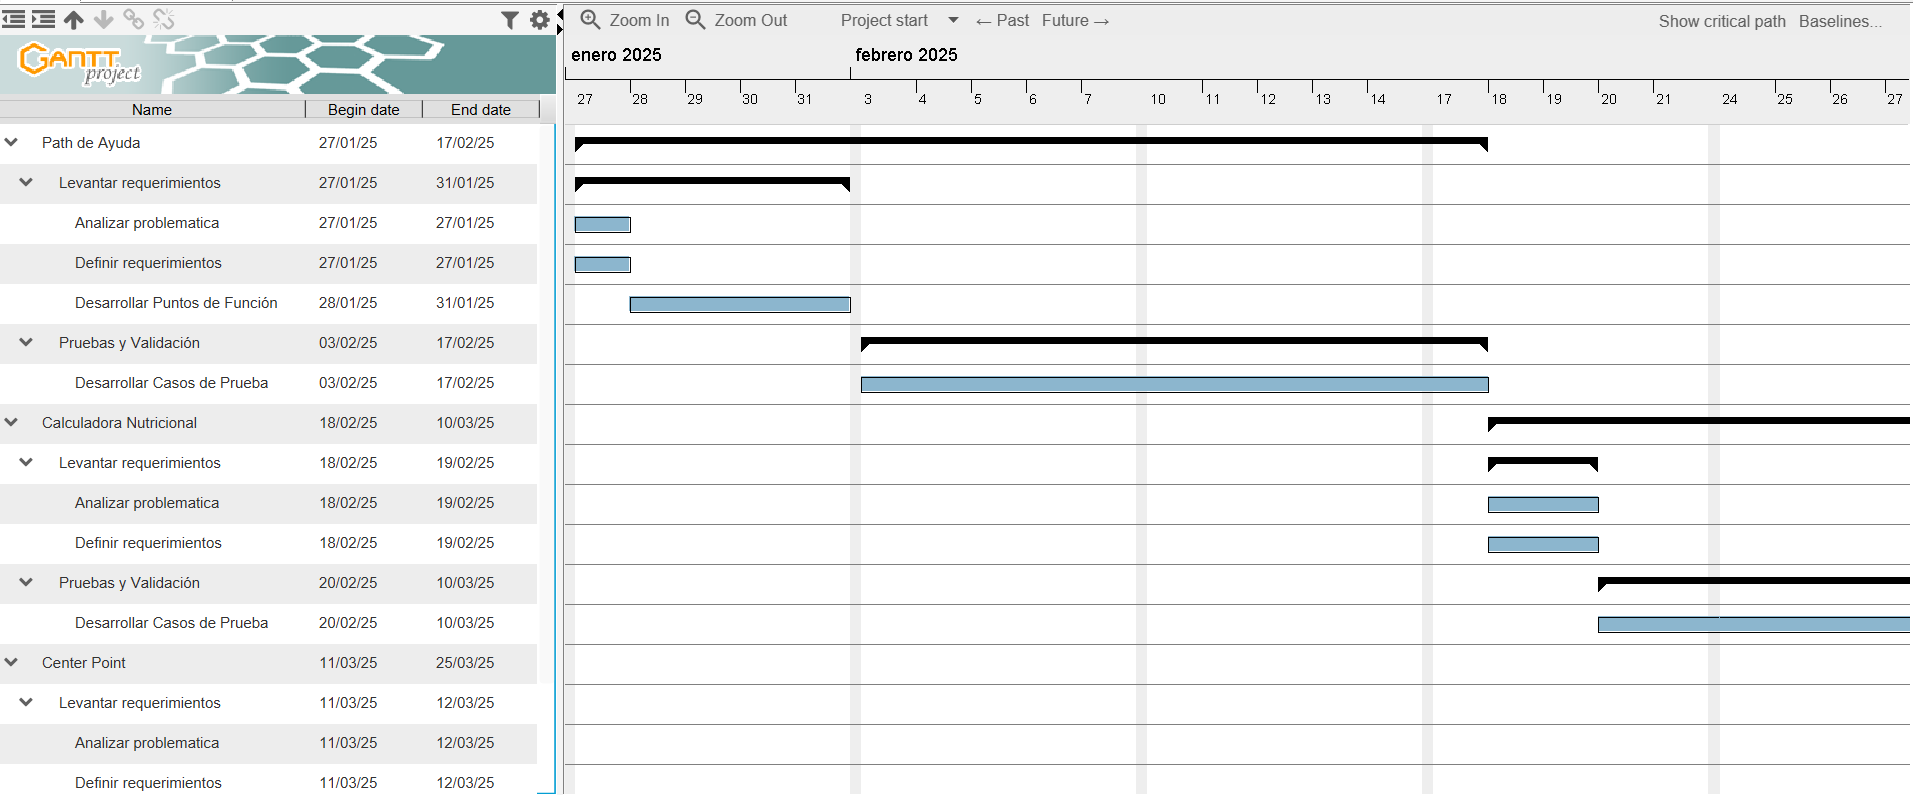
\includegraphics[width=1.0\textwidth]
		{Imagenes/Planeacion/EneFeb.png}
		\caption{Planeación de actividades del mes de Enero y Febrero
		}\label{a2}
	\end{figure}
	
	\begin{figure}[H]
		\centering
		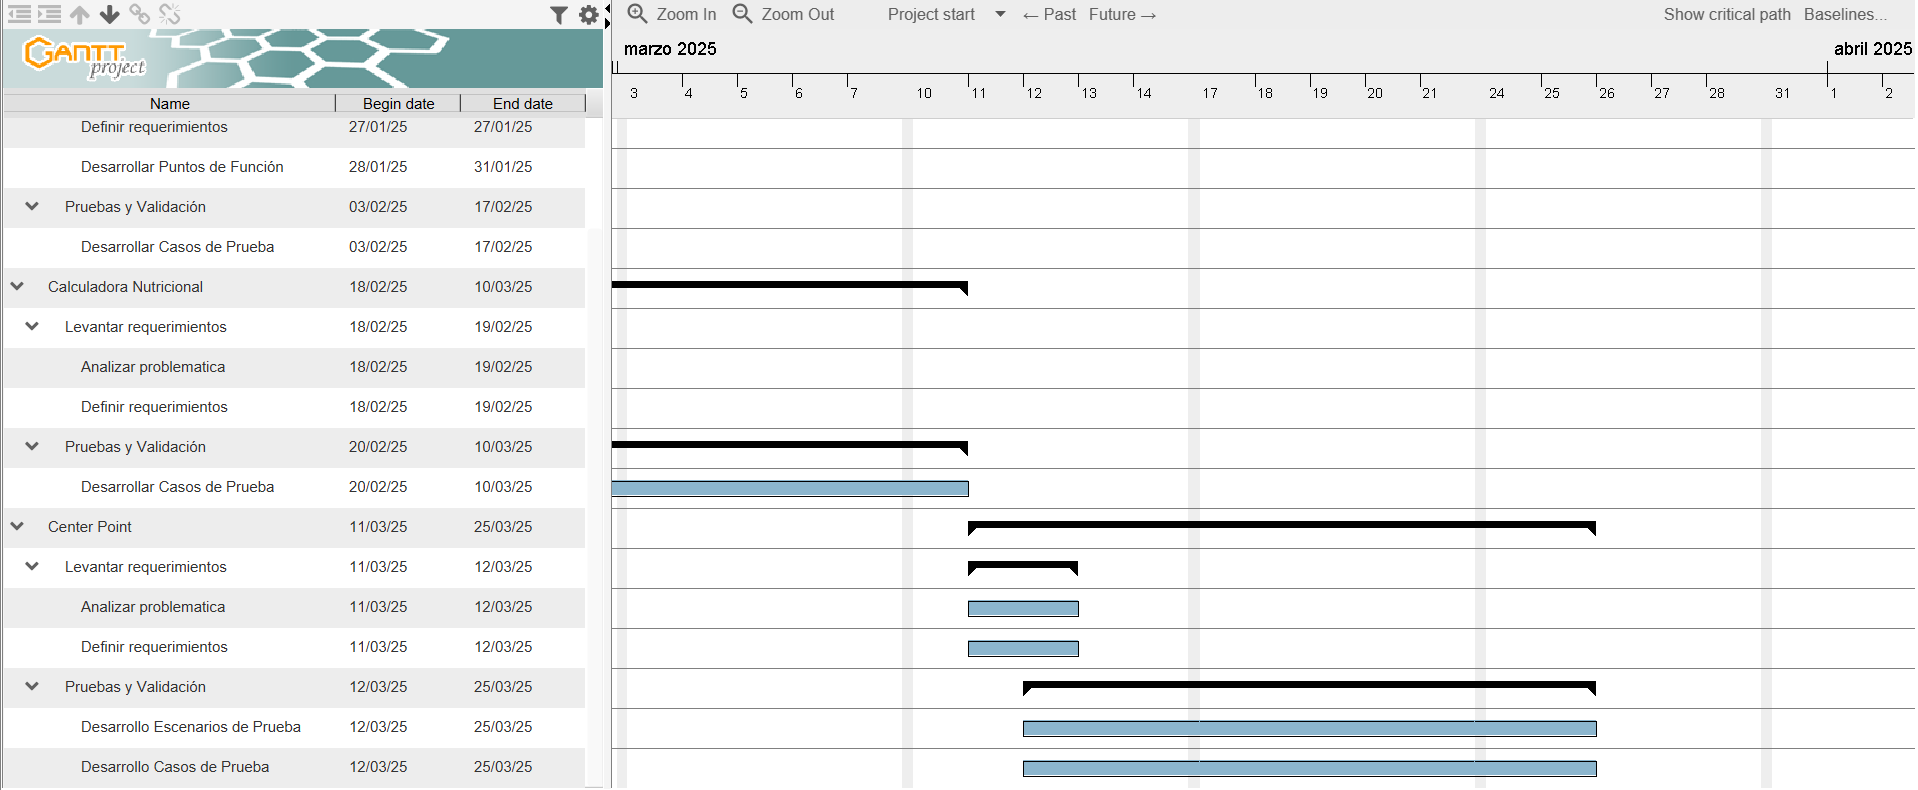
\includegraphics[width=1.0\textwidth]
		{Imagenes/Planeacion/Mar.png}
		\caption{Planeación de actividades del mes de Marzo
		}\label{a2}
	\end{figure}


%CAPITULO MARCO TEÓRICO: bases teorícas del proyecto. conceptos básicos y antecedentes o información existente.
%____________________________________________________________________________________________________________________
	
\chapter{Marco Teórico}
\newpage

La administración de proyectos de software es un proceso que integra metodologías y técnicas para la planificación, programación, ejecución y seguimiento de proyectos de desarrollo. Su principal objetivo es optimizar el trabajo de los desarrolladores mediante una adecuada gestión de recursos, garantizando que el proyecto se lleve a cabo de manera eficiente y productiva. Además, permite minimizar los riesgos asociados y responder de manera efectiva ante cualquier dificultad que pueda surgir en el proceso de desarrollo (Tiffin University, 2024). \\

Dentro de la administración de proyectos, la planificación juega un papel fundamental, ya que define el rumbo del proyecto desde su concepción hasta su finalización. En esta fase, se establecen los alcances, se asignan los recursos necesarios, se diseña un cronograma de ejecución y se implementan estrategias de comunicación. Asimismo, se consideran elementos clave como las pruebas y el mantenimiento del software, garantizando su correcto funcionamiento y su sostenibilidad a lo largo del tiempo (Wrike, 2024).\\

Otro aspecto esencial en el desarrollo de software es la documentación, pues permite estructurar y registrar la información clave del proyecto. A pesar de su importancia, en muchas ocasiones es percibida como una tarea que resta tiempo productivo. Sin embargo, la ausencia de documentación adecuada puede dificultar la comprensión del sistema, limitar su escalabilidad y complicar su mantenimiento a largo plazo. La documentación puede incluir especificaciones funcionales, diagramas de casos de uso y mockups de interfaces, entre otros elementos que faciliten el desarrollo y la futura gestión del software (Arsys, 2024).\\

La gestión de requisitos es otro pilar clave en la administración de proyectos de software, ya que permite definir, analizar, priorizar y validar las necesidades del sistema. Para ello, se elabora un Plan de Gestión de Requisitos (RMP), el cual establece los procesos de recopilación, documentación y control de requisitos a lo largo del ciclo de vida del proyecto. Este enfoque permite garantizar que el producto final cumpla con las expectativas del cliente y los estándares de calidad, al tiempo que facilita la detección temprana de errores y contribuye a la reducción de costos y riesgos (IBM, 2024).\\

Además de la planificación y gestión de requisitos, el Análisis de Puntos de Función (FPA, por sus siglas en inglés) se ha convertido en una herramienta fundamental en la medición de la funcionalidad de un sistema de software. Este enfoque permite cuantificar el tamaño de un proyecto con base en elementos como datos procesados, tipos de transacciones y consultas realizadas. A partir de esta información, los desarrolladores pueden identificar áreas que requieren optimización y realizar análisis comparativos de rendimiento con relación a estándares de la industria (BlueOptima, 2024).\\

El FPA también resulta útil para estimar el tiempo y los recursos necesarios en el desarrollo de un proyecto, lo que facilita una planificación más precisa y una gestión más eficiente del proceso. Su aplicación permite evaluar la productividad del equipo, monitorear el progreso del proyecto y mejorar el análisis de costo-beneficio, asegurando que las decisiones sobre inversiones y asignación de recursos se tomen de manera fundamentada. Además, contribuye a alinear los esfuerzos de desarrollo con los objetivos estratégicos de la organización, garantizando que el software desarrollado genere valor a los usuarios finales (GeeksForGeeks, 2024).\\


Las pruebas de software son un proceso esencial en el desarrollo de aplicaciones, cuyo objetivo principal es evaluar su funcionalidad e identificar posibles errores antes de su implementación final. Según Certus (2022), << este proceso garantiza que el software cumpla con los estándares de calidad y que el producto entregado sea confiable y eficiente>>.\\

En la industria del software, el aseguramiento de calidad (QA) y las pruebas forman una parte crucial del ciclo de vida del desarrollo de software (SDLC). IBM (2023) señala que defectos en el software pueden dañar la reputación de una empresa, frustrar a los clientes e incluso generar pérdidas económicas significativas. Por ello, el control de calidad es indispensable para evitar retrasos en las entregas y garantizar el funcionamiento óptimo de los sistemas.\\

El control de calidad en el desarrollo de software se implementa a través de un procedimiento metódico que supervisa y revisa cada etapa del desarrollo. BrowerStack (2023) destaca que este proceso incluye actividades como análisis de requisitos, preparación de pruebas, ejecución de pruebas, seguimiento de defectos y redacción de informes.\\

IBM (2023) resalta que la tendencia actual en la industria es realizar pruebas continuas, es decir, iniciar las pruebas desde la fase de diseño, continuar con ellas durante el desarrollo y mantenerlas incluso en producción. Este enfoque permite detectar errores con mayor anticipación y mejorar la calidad del producto final.\\

Para logar una validación integral del software, es fundamental definir correctamente los escenarios y casos de prueba. Leapwork (2025) los describe de la siguiente manera. "Los escenarios de prueba es un documento de alto nivel que describe la funcionalidad que se evaluará, proporcionando una visión general de lo que debe probarse. Se centra en el comportamiento de software sin entrar en detalles específicos."\\

Los casos de prueba son un conjunto de condiciones o variables específicas que permiten evaluar si un sistema cumple con los requisitos establecidos. Incluyendo entradas, condiciones, procedimiento y resultados esperado, guiando al evaluador paso a paso.\\

La correcta implementación de estos elementos permite asegurar el correcto funcionamiento del software en diversas situaciones y garantizar un producto de alta calidad. Como afirma IBM (2023), las pruebas continuas y bien estructuradas contribuyen a minimizar riesgos y mejorar la satisfacción del usuario final, optimizando el rendimiento de las aplicaciones en un mercado altamente competitivo.\\

En la actualidad, las empresas enfrentan un entorno de negocios cada vez más 
competitivo y volátil. Las expectativas de los clientes son cada vez más altas, y la necesidad de ser flexibles, eficientes y capaces de adaptarse rápidamente a los cambios en el mercado es más crucial que nunca. En este contexto, la mejora de procesos se ha convertido en una prioridad para muchas organizaciones, ya que optimizar los procesos internos puede llevar a una reducción de costos, una mayor eficiencia, mejor calidad y, en última instancia, un mayor nivel de satisfacción del cliente (Jacobs, 2006). \\

Tradicionalmente, la mejora de procesos se ha abordado mediante métodos rígidos y estructurados que a menudo son lentos y difíciles de adaptar a las condiciones cambiantes del mercado. Sin embargo, las metodologías ágiles, originadas en el desarrollo de software, han demostrado ser una alternativa eficaz para acelerar la mejora de procesos, al proporcionar un marco más flexible, iterativo y adaptable. Las técnicas ágiles no solo facilitan la mejora continua de los procesos, sino que también permiten que las organizaciones respondan de manera rápida y eficiente a los cambios que surgen tanto a nivel interno como externo (Jacobs, 2006).\\

La mejora de procesos se refiere a un enfoque sistemático para hacer que los procesos dentro de una organización sean más eficientes y efectivos, buscando no solo la optimización de la producción, sino también la creación de valor para el cliente. Sin embargo, en muchas metodologías tradicionales, el proceso de mejora es lineal y se centra en soluciones de largo plazo que pueden ser difíciles de implementar rápidamente y que no se adaptan bien a las necesidades cambiantes (Jacobs, 2006).\\

Las metodologías ágiles ofrecen un enfoque totalmente diferente. En lugar de implementar mejoras grandes y complejas de una sola vez, las metodologías ágiles se centran en realizar mejoras rápidas e iterativas a lo largo del tiempo. Estas mejoras, aunque más pequeñas en escala, son frecuentes y se basan en un ciclo continuo de retroalimentación y evaluación. Esto permite a las organizaciones implementar cambios rápidamente, probarlos, evaluarlos y ajustarlos según sea necesario, lo que acelera la mejora de los procesos y reduce el riesgo de error (Jacobs, 2006).\\

Uno de los pilares fundamentales de las metodologías ágiles es el ciclo iterativo de trabajo. En lugar de seguir un enfoque de “todo o nada”, las organizaciones adoptan ciclos cortos y definidos de trabajo, llamados "sprints" o iteraciones, durante los cuales se desarrollan, prueban y mejoran los procesos. Estos ciclos pueden durar desde unas pocas semanas 
hasta un mes, y en cada uno de ellos se realizan pequeñas mejoras en los procesos existentes. Al final de cada iteración, se recoge retroalimentación tanto de los empleados involucrados como de los clientes, lo que permite realizar ajustes rápidos y ajustar el rumbo cuando es necesario (Jacobs, 2006).\\

En las metodologías ágiles, la colaboración es esencial. A diferencia de los enfoques tradicionales, que a menudo operan en silos, las metodologías ágiles promueven el trabajo conjunto entre diferentes departamentos y equipos. Esta colaboración se extiende no solo dentro de la organización, sino también con los clientes y otras partes interesadas. Las reuniones diarias, conocidas como "scrums", y las revisiones periódicas permiten que 
todos los involucrados se mantengan alineados con los objetivos y compartan su perspectiva sobre el progreso de las mejoras (Jacobs, 2006).\\

La visibilidad es otro principio central de las metodologías ágiles. En lugar de ocultar el progreso y las métricas del equipo, las metodologías ágiles fomentan la transparencia a través de herramientas como tableros visuales (por ejemplo, Kanban). Estos tableros permiten a todos los miembros del equipo ver en tiempo real el estado de las tareas y los procesos en curso, lo que fomenta la responsabilidad y la colaboración (Jacobs, 2006).\\

En un entorno de negocios caracterizado por la incertidumbre y la rapidez de los cambios, la capacidad de adaptarse rápidamente es crucial. Las metodologías ágiles permiten que las organizaciones sean más flexibles, ya que no están atadas a un plan rígido de mejora de procesos a largo plazo. En lugar de seguir un enfoque predefinido, las organizaciones pueden modificar y ajustar sus procesos en función de la evolución del mercado, las nuevas tecnologías o las solicitudes de los clientes. Esta capacidad para adaptarse 
rápidamente a nuevas situaciones reduce el riesgo de implementar soluciones ineficaces y permite a las organizaciones mantenerse competitivas en un mercado en constante cambio (Jacobs, 2006).\\

Scrum es una de las metodologías ágiles más populares y se utiliza para la mejora de procesos mediante ciclos cortos y planificados de trabajo. Un equipo Scrum se organiza en torno a roles como el Product Owner, el Scrum Master y el equipo de desarrollo, y se enfoca en completar un conjunto específico de tareas durante cada iteración. Al final de cada sprint, se realiza una revisión y retrospectiva, donde se evalúa el progreso realizado 
y se ajustan las tareas para la siguiente iteración. Esta estructura permite una mejora continua y una adaptación rápida a los cambios en el entorno de trabajo (Jacobs, 2006).\\

Kanban es una técnica visual utilizada para gestionar el flujo de trabajo de manera eficiente. Mediante el uso de un tablero visual, los equipos pueden gestionar y optimizar el flujo de tareas a través de diferentes etapas, asegurando que no se acumulen cuellos de botella y que los procesos se mantengan fluidos. Kanban es particularmente útil para la mejora continua, ya que permite realizar ajustes rápidos y específicos en función de los cuellos de botella identificados, lo que reduce el tiempo de espera y mejora la eficiencia del proceso (Jacobs, 2006).\\

Lean es una filosofía de mejora de procesos que se centra en la eliminación del desperdicio y la creación de valor para el cliente. En lugar de centrarse exclusivamente en la eficiencia, Lean también pone énfasis en mejorar la experiencia del cliente y eliminar todas las actividades que no aportan valor. A través de técnicas como la mejora continua (Kaizen) y la eliminación de actividades innecesarias, las organizaciones pueden optimizar 
sus procesos y hacer un uso más eficiente de sus recursos (Jacobs, 2006).\\

El diseño de frameworks, especialmente en el desarrollo de software, es uno de los aspectos clave para garantizar la eficiencia, escalabilidad y mantenibilidad de una solución tecnológica. Un framework bien diseñado proporciona una estructura flexible y reutilizable que facilita el desarrollo de aplicaciones, ahorrando tiempo y esfuerzo a los desarrolladores. Sin embargo, la creación de un framework no es una tarea sencilla, ya que requiere un equilibrio entre simplicidad, extensibilidad y facilidad de uso. Las directrices para el diseño de frameworks buscan proporcionar principios y buenas prácticas que guíen a los desarrolladores en la creación de frameworks robustos y efectivos (Cwalina \& Abrams, 2006).\\

Un framework es, en esencia, una plataforma de soporte sobre la cual los desarrolladores pueden construir aplicaciones. A diferencia de una biblioteca, que proporciona funcionalidades que el programador invoca, un framework define la estructura básica de la aplicación y dicta el flujo del control. Esto hace que el diseño de un framework sea una tarea crucial, ya que influye directamente en cómo los desarrolladores utilizarán las herramientas y los componentes de la aplicación (Cwalina \& Abrams, 2006).\\

Para garantizar que un framework sea eficaz, debe seguir ciertas directrices que aseguren su robustez, flexibilidad y facilidad de uso.\\

Uno de los conceptos más importantes en el diseño de frameworks es la inversión de control. A diferencia de una aplicación tradicional donde el flujo de control es manejado por el programador, en un framework, el control es invertido. Esto significa que el framework define el flujo general de la aplicación y el desarrollador proporciona solo los componentes específicos. Este patrón es esencial en el diseño de frameworks, ya que permite que el 
framework sea flexible y reutilizable en diferentes contextos. En otras palabras, el framework establece el marco general de la aplicación, mientras que los desarrolladores se enfocan en implementar solo las partes que son relevantes para su proyecto (Cwalina \& Abrams, 2006).\\

Un framework debe ser fácil de usar y proporcionar una interfaz clara y sencilla. La complejidad en un framework puede dificultar su adopción y aumentar la curva de aprendizaje para los desarrolladores. Para lograr una interfaz sencilla, es esencial que el framework esté diseñado con la facilidad de integración y comprensión en mente. Los desarrolladores deben poder integrar el framework en su proyecto sin esfuerzo adicional, y 
las APIs deben ser intuitivas. Para ello, la documentación completa y detallada es crucial, pues ayuda a los desarrolladores a comprender el propósito de cada componente y cómo utilizarlo correctamente (Cwalina \& Abrams, 2006). \\

Un framework debe permitir a los desarrolladores trabajar con un nivel adecuado de abstracción. Esto significa que los desarrolladores deben poder concentrarse en el diseño y la lógica de su aplicación sin preocuparse por los detalles de implementación subyacentes. Sin embargo, un buen framework debe permitir la extensión de sus funcionalidades sin que esto signifique alterar la estructura básica del framework. La flexibilidad es fundamental, ya que el framework debe ser capaz de adaptarse a las necesidades cambiantes de las aplicaciones que se desarrollan sobre él (Cwalina \& Abrams, 2006).\\

Un marco de trabajo eficaz debe permitir la reutilización de componentes en diversos proyectos y escenarios. Para lograr esto, es necesario que los componentes sean modulares y autónomos, de modo que puedan ser fácilmente reemplazados o mejorados sin afectar el resto del sistema. La modularidad no solo facilita la reutilización, sino que también mejora la mantenibilidad del código, ya que cualquier modificación o actualización de un módulo específico no afectará el comportamiento de otros módulos del sistema (Cwalina \& Abrams, 2006).\\

Las convenciones y normas consistentes son esenciales en el diseño de frameworks. Esto asegura que los desarrolladores sigan un conjunto común de reglas y principios al utilizar el framework, lo que aumenta la coherencia y facilita la comprensión del código. Las convenciones pueden incluir nombres de clases, estructuras de carpetas y patrones de diseño. Si un framework tiene un conjunto claro de convenciones, los desarrolladores pueden aprender rápidamente cómo utilizarlo y trabajar de manera más eficiente (Cwalina 
\& Abrams, 2006).\\

Un framework debe ser escalable para poder adaptarse a la evolución del software a lo largo del tiempo. Esto incluye no solo la capacidad de manejar mayores cargas de trabajo o nuevos requisitos, sino también la capacidad de ser modificado sin generar efectos secundarios imprevistos. La mantenibilidad es igualmente crítica; el diseño del framework debe ser tal que, en caso de errores o necesidades de actualización, el código pueda ser 
modificado sin dificultad. Los patrones de diseño y la modularidad también juegan un papel importante en este aspecto, pues garantizan que las actualizaciones sean fáciles de implementar sin romper otras partes del sistema (Cwalina \& Abrams, 2006).\\

El desacoplamiento se refiere a la capacidad de un framework para minimizar las dependencias entre los componentes. Un framework bien diseñado reduce la 
interdependencia entre sus módulos, lo que permite a los desarrolladores modificar o reemplazar componentes individuales sin afectar otras áreas del sistema. Este desacoplamiento permite un mayor control sobre el sistema y facilita el mantenimiento a largo plazo. Además, permite a los desarrolladores integrar otros sistemas o tecnologías en el futuro sin que haya problemas de compatibilidad (Cwalina \& Abrams, 2006).\\

El patrón MVC es ampliamente utilizado en el diseño de frameworks, especialmente en el desarrollo de aplicaciones web. En este patrón, se separa la lógica de la aplicación en tres componentes principales: el Modelo (que maneja los datos), la Vista (que se encarga de la presentación) y el Controlador (que gestiona las interacciones entre el Modelo y la Vista). 
Este patrón ayuda a separar las preocupaciones dentro del código, lo que facilita la mantenibilidad y la extensibilidad del framework. Al utilizar MVC, los desarrolladores pueden modificar la presentación de la aplicación sin afectar la lógica de negocio y viceversa (Cwalina \& Abrams, 2006).\\

El patrón de fábrica es útil cuando se necesita crear objetos sin especificar exactamente qué clase de objeto se va a crear. En el contexto de un framework, este patrón permite que los desarrolladores creen instancias de clases de forma flexible sin tener que preocuparse por las clases exactas que se están utilizando. El patrón de fábrica proporciona una interfaz común para crear objetos, lo que mejora la modularidad y la reutilización del 
código dentro del framework (Cwalina \& Abrams, 2006).\\

El patrón Singleton asegura que una clase tenga solo una instancia en todo el sistema y proporciona un punto de acceso global a esa instancia. En el contexto de un framework, este patrón es útil cuando se necesita asegurar que ciertos recursos, como bases de datos o configuraciones, sean compartidos entre todas las instancias de una aplicación. El Singleton ayuda a evitar la creación de múltiples instancias innecesarias y mejora la eficiencia del framework (Cwalina \& Abrams, 2006).\\

El patrón de estrategia permite cambiar el comportamiento de un objeto en tiempo de ejecución, lo que es útil cuando el comportamiento del framework necesita ser flexible. A través de este patrón, los desarrolladores pueden definir una familia de algoritmos o estrategias que puedan ser intercambiados según sea necesario. Esto mejora la extensibilidad del framework, permitiendo que el comportamiento del sistema sea modificado sin afectar la estructura subyacente (Cwalina \& Abrams, 2006).\\

El patrón de adaptador permite que un sistema utilice interfaces incompatibles sin modificar el código existente. En el contexto de un framework, este patrón es útil cuando se integra con sistemas externos que no siguen las mismas convenciones o estructuras. El adaptador convierte las interfaces de los sistemas externos en una forma que sea compatible con el framework, lo que facilita la integración de nuevas tecnologías sin afectar la arquitectura general (Cwalina \& Abrams, 2006).\\

Un framework bien diseñado permite a los desarrolladores centrarse en la lógica de negocio y la funcionalidad específica, sin tener que reinventar la rueda. Al proporcionar componentes reutilizables y un conjunto de directrices claras, un framework mejora la productividad, ya que los desarrolladores no necesitan comenzar desde cero para cada nuevo proyecto (Cwalina \& Abrams, 2006).\\

Un framework diseñado siguiendo las mejores prácticas y 
principios sólidos tiende a ser más estable y menos propenso a errores. Al 
proporcionar una estructura predefinida y simplificada, los desarrolladores tienen menos oportunidades para cometer errores y, cuando estos ocurren, son más fáciles de localizar y corregir (Cwalina \& Abrams, 2006).\\

Un framework bien diseñado mejora la calidad del software al garantizar que los desarrolladores sigan las mejores prácticas y patrones de diseño. La consistencia y la modularidad inherentes a un buen framework también conducen a un código más limpio, entendible y fácil de mantener, lo que mejora la calidad general del software (Cwalina \& Abrams, 2006).\\

Un framework que se ha diseñado con la flexibilidad y 
escalabilidad en mente permite a las aplicaciones crecer sin problemas a medida que aumentan los requisitos. La modularidad y la capacidad de extensión facilitan la integración de nuevas funcionalidades y la adaptación a necesidades cambiantes (Cwalina \& Abrams, 2006).\\

BPMN (Business Process Model and Notation) es una notación gráfica ampliamente utilizada para representar los procesos de negocio en una forma estandarizada y comprensible tanto para los desarrolladores como para los analistas de negocio. Su propósito es proporcionar una forma intuitiva y visual de documentar los procesos empresariales, con el fin de facilitar la comprensión, la comunicación y la mejora continua de los procesos. El uso de BPMN ha crecido significativamente en el ámbito de la gestión de procesos de negocio (BPM), especialmente por su capacidad para representar flujos de trabajo complejos, interacciones entre actores y la toma de decisiones a lo largo de un proceso empresarial (Freund, Rucker, \& Hitpass, 2017).\\

El BPMN, como estándar, busca ser un puente entre las necesidades del negocio y las soluciones tecnológicas, permitiendo que los procesos sean modelados y luego ejecutados a través de herramientas y plataformas de BPM. Este marco teórico se centra en los principios fundamentales, elementos y beneficios del uso de BPMN en el diseño y la mejora de procesos de negocio, así como en su aplicación práctica (Freund, Rucker, \& Hitpass, 2017).\\

El principal objetivo de BPMN es proporcionar una notación estándar 
que permita a los analistas de negocio, diseñadores, desarrolladores y cualquier otra persona involucrada en la gestión de procesos comprender y visualizar cómo se desarrollan los procesos dentro de una organización. Esto ayuda no solo en la documentación y análisis de los procesos actuales, sino también en la mejora continua y la optimización de estos procesos. BPMN logra esto mediante una notación gráfica que describe las secuencias, eventos, actividades y decisiones dentro de un proceso (Freund, Rucker, \& Hitpass, 2017).\\

La notación gráfica de BPMN es simple y visualmente clara, lo que 
facilita la comprensión de los procesos de negocio sin necesidad de una gran formación técnica (Freund, Rucker, \& Hitpass, 2017).\\

La utilización de BPMN no solo se limita al modelado de 
procesos, sino que también es una herramienta esencial para la automatización de procesos empresariales. Una vez que se ha modelado un proceso de negocio en BPMN, este puede ser implementado y ejecutado en una plataforma de BPM, lo que permite automatizar la secuencia de actividades, la toma de decisiones y la gestión de excepciones (Freund, Rucker, \& Hitpass, 2017).\\

Al usar BPMN, las organizaciones pueden garantizar que 
todos los procesos estén modelados de acuerdo con un estándar común, lo que mejora la comunicación y la comprensión en toda la empresa (Freund, Rucker, \& Hitpass, 2017).\\

El marco ágil es una metodología que permite a las organizaciones desarrollar productos de manera iterativa e incremental, manteniendo una alta flexibilidad frente a los cambios del mercado. El Scaled Agile Framework (SAFe) es una implementación de las prácticas ágiles a gran escala, diseñada para permitir a las organizaciones manejar proyectos 
complejos de gran tamaño, donde múltiples equipos ágiles deben colaborar para lograr un objetivo común. A medida que las organizaciones crecen y sus necesidades se vuelven más complejas, es crucial adoptar metodologías que no solo promuevan la agilidad dentro de los equipos individuales, sino también entre equipos y a nivel organizacional (Knaster \& 
Leffingwell, 2020).\\

El Scaled Agile Framework (SAFe), en su versión más reciente, proporciona una estructura robusta y escalable que permite a las empresas adoptar agilidad de manera efectiva, gestionando la interdependencia entre equipos ágiles, integrando todas las partes del negocio y asegurando que la organización funcione de manera más rápida y flexible. SAFe es particularmente útil para las organizaciones grandes, en las que los proyectos abarcan múltiples equipos, departamentos y ubicaciones geográficas (Knaster \& Leffingwell, 2020).\\

SAFe es un conjunto de principios y prácticas basados en los métodos ágiles que se utilizan para coordinar, ejecutar y entregar proyectos complejos en entornos empresariales grandes. SAFe es un marco de trabajo que abarca varios niveles organizativos: equipo, programa, solución y cartera. Cada nivel tiene su propio conjunto de prácticas ágiles, pero todos están alineados con los mismos principios subyacentes de agilidad, transparencia, colaboración y entrega continua (Knaster \& Leffingwell, 2020).\\

El Static Application Security Testing (SAST) es un enfoque de prueba de seguridad que analiza el código fuente de una aplicación mientras está en reposo, sin ejecutar el programa. Se enfoca en encontrar vulnerabilidades de seguridad en el código antes de que se ejecute, lo que permite detectar fallos en la fase de desarrollo. El análisis SAST examina el código estático para identificar posibles vulnerabilidades como inyecciones SQL, desbordamientos de búfer, exposición de información sensible y otros problemas que podrían comprometer la seguridad de la aplicación (Chess \& West, 2007).\\

El Dynamic Application Security Testing (DAST) es un enfoque de prueba de seguridad que se lleva a cabo mientras la aplicación está en ejecución. A diferencia del SAST, DAST no analiza el código fuente directamente, sino que interactúa con la aplicación de manera similar a un atacante, probando vulnerabilidades de seguridad durante la ejecución en un entorno real o simulado. Este tipo de pruebas es útil para identificar vulnerabilidades que 
no se pueden detectar a través de análisis estático, como problemas de configuración, exposición de servicios inseguros o errores de implementación (Vieira et al., 2019).\\

Ambos enfoques, SAST y DAST, son fundamentales en el proceso de pruebas de 
seguridad de aplicaciones, pero cada uno tiene sus fortalezas y limitaciones. Mientras que SAST se enfoca en encontrar vulnerabilidades dentro del código estático desde el inicio del ciclo de vida del desarrollo, DAST evalúa la seguridad de la aplicación en tiempo real, detectando problemas que solo se pueden identificar cuando la aplicación está en funcionamiento.\\

La integración de ambos enfoques puede proporcionar una cobertura de seguridad más completa. SAST es útil para identificar vulnerabilidades a nivel de código, mientras que DAST es esencial para probar cómo la aplicación interactúa con su entorno operativo. Una estrategia combinada de ambos tipos de pruebas ayuda a garantizar una mayor seguridad 
en las aplicaciones, reduciendo tanto los riesgos durante el desarrollo como los que pueden surgir una vez que el software está en producción.\\

%CAPITULO DESARROLLO DEL PROYECTO: procedimiento o descripci�n de las actividades realizadas, como es un desarrollo es importante
%____________________________________________________________________________________________________________________


\chapter{Desarrollo del Proyecto}
\newpage
	
\section{Path de ayuda}

	El proyecto Path de Ayuda está diseñado para mejorar la eficiencia en la planta de Formas Sólidas, proporcionando un sistema de monitoreo en tiempo real que facilite la gestión del proceso de fabricación. Este sistema permitirá visualizar el avance de los lotes en cada línea de producción y gestionar alertas sobre posibles fallas, notificando a los dispositivos vinculados del personal responsable.\\
	
	Se participó en la fase inicial del proyecto, enfocándose en la documentación necesaria para su desarrollo. Dado que la implementación del sistema sería realizada por una empresa externa, nuestra labor consistió en estructurar la información clave, garantizar una base organizada y clara para su desarrollo.\\
	
	El resultado fue una adecuada organización del proyecto, facilitando la transición hacia el equipo de desarrollo externo y asegurando que las necesidades del negocio fueran correctamente traducidas en especificaciones técnicas.

\subsection{Levantamiento de requerimeintos}

	Para garantizar que el proyecto Path de Ayuda cumpliera con las necesidades operativas de la planta de Formas Sólidas, llevamos a cabo un proceso de levantamiento de requerimientos con el objetivo de documentar de manera precisa las funcionalidades y características esenciales del sistema.\\
	
	Durante este proceso, uno de los mayores desafíos fue traducir las necesidades operativas en especificaciones técnicas claras, asegurando que el sistema cumpliera con los estándares requeridos.\\
	
	Gracias a este levantamiento de información, el equipo de desarrollo externo pudo contar con una documentación estructurada y detallada, facilitando la implementación del sistema y asegurando que el producto final estuviera alineado con los objetivos de la organización.

\subsection{Descripción de Épicas}

	Como parte de la documentación para el desarrollo del sistema Path de Ayuda, se llevó a cabo la definición y estructuración de las épicas del proyecto, aplicando principios de metodologías ágiles como Scrum. Estas épicas representan un conjunto de funcionalidades de alto nivel que permiten organizar el trabajo en historias de usuario más detalladas, facilitando la planificación, ejecución y gestión eficiente del desarrollo.\\
	
	Siguiendo el marco de Scrum, cada épica fue desglosada en historias de usuario, las cuales se priorizaron dentro del backlog del sistema. Esta estrategia permitió estructurar el desarrollo de un flujo de trabajo adaptable a los cambios y necesidades del usuario. Además, este enfoque promovió una entrega incremental del sistema, permitiendo validar y ajustar los requerimientos a lo largo del proceso para garantizar una implementación alineada con los objetivos del proyecto.\\
	
	Para garantizar una documentación clara y estandarizada, cada épica fue documentada en un formato estructurado de la siguiente manera:\\
		
	{\leftskip=1em 
		\noindent 
		1. Título de la Épica – Nombre que resume su propósito.
	\par}
	
	{\leftskip=1em 
		\noindent 
		2. Descripción – Explicación detallada de la funcionalidad y su importancia.
	\par}
	
	{\leftskip=1em 
		\noindent 
		3. Criterios de Aceptación – Reglas y condiciones necesarias para que la épica se considere completada.\\
	\par}
	
\subsection{Puntos de Función}

	Como parte del proceso de documentación del proyecto Path de Ayuda, se realizó un Análisis de Punto de Función (FPA) para estimar el tamaño del software y evaluar el esfuerzo necesario para su desarrollo. Esta técnica permitió cuantificar las funcionalidades del sistema basándose en la perspectiva del usuario, facilitando una mejor planificación del proyecto y una estimación más precisa de costos y tiempos de desarrollo.\\
	
	Para llevar a cabo el análisis, se identificaron y clasificaron los siguientes elementos del sistema:\\
	
	{\leftskip=1em 
	  \noindent 
		1.Entradas Externas (EI) – Datos ingresados por los usuarios en el sistema.
	\par}
	
	{\leftskip=1em 
	  \noindent 
		2.Salidas Externas (EO) – Información generada y presentada a los usuarios.
	\par}
	
	{\leftskip=1em 
	  \noindent 
		3.Consultas Externas (EQ) – Procesos que permiten a los usuarios recuperar información específica
	\par}

	{\leftskip=1em 
	  \noindent 
		4.Archivos Lógicos Internos (ILF) – Bases de datos o archivos que almacenan información persistente.
	\par}

	\begin{figure}[htp]
		\centering
		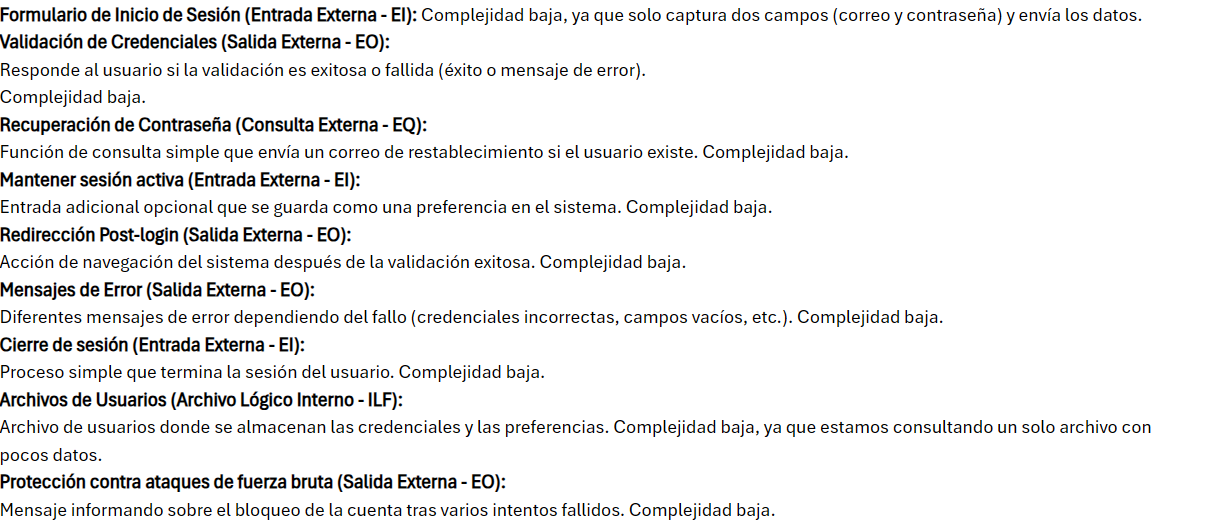
\includegraphics[width=1.0\textwidth]
		{Imagenes/PathAyuda/FpsLogin.png}
		\caption{Puntos de Función - Login}\label{a1}
	\end{figure}
	
	\begin{figure}[H]
		\centering
		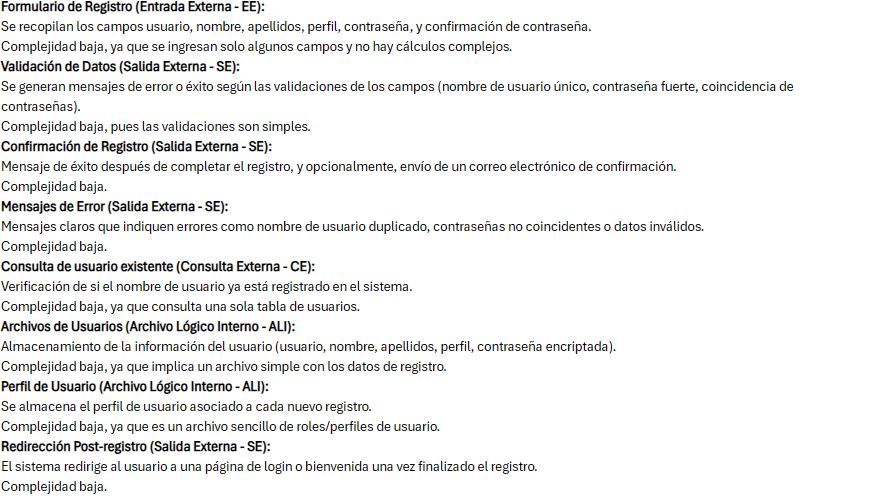
\includegraphics[width=1.0\textwidth]
		{Imagenes/PathAyuda/FpsRegistroUsuario.png}
		\caption{Puntos de Función - Registo de Usuarios}\label{a2}
	\end{figure}

	\begin{figure}[H]
		\centering
		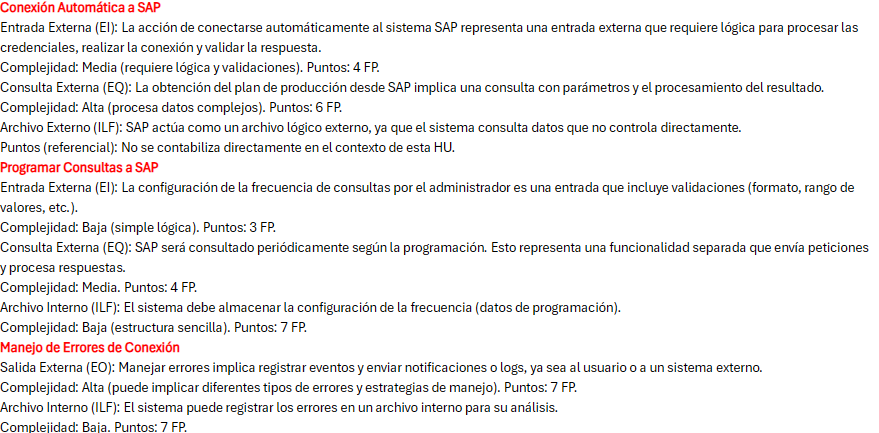
\includegraphics[width=1.0\textwidth]
		{Imagenes/PathAyuda/FpsIntegracionSAP.png}
		\caption{Puntos de Función - Integración de SAP}\label{a2}
	\end{figure}

	\begin{figure}[H]
		\centering
		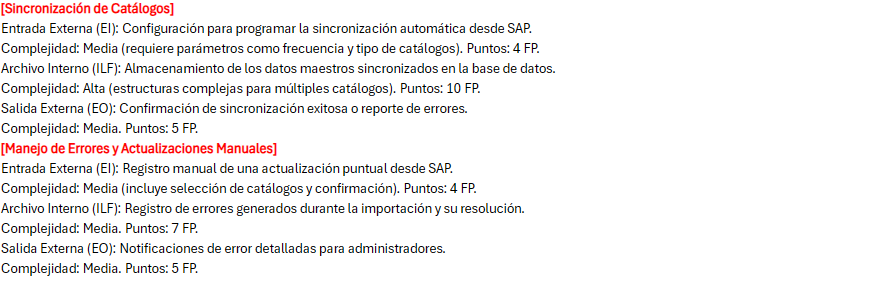
\includegraphics[width=1.0\textwidth]
		{Imagenes/PathAyuda/FpsCatalagoSAP.png}
		\caption{Puntos de Función - Catalagos SAP}\label{a2}
	\end{figure}
	
	\begin{figure}[H]
		\centering
		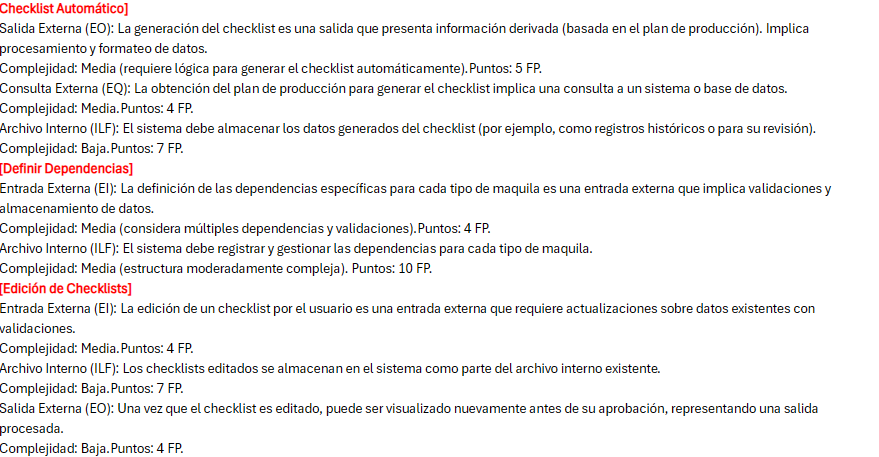
\includegraphics[width=1.0\textwidth]
		{Imagenes/PathAyuda/FpsDependeciasChecklist.png}
		\caption{Puntos de Función - Gestión de Checklist
		}\label{a2}
	\end{figure}
	
	\begin{figure}[H]
		\centering
		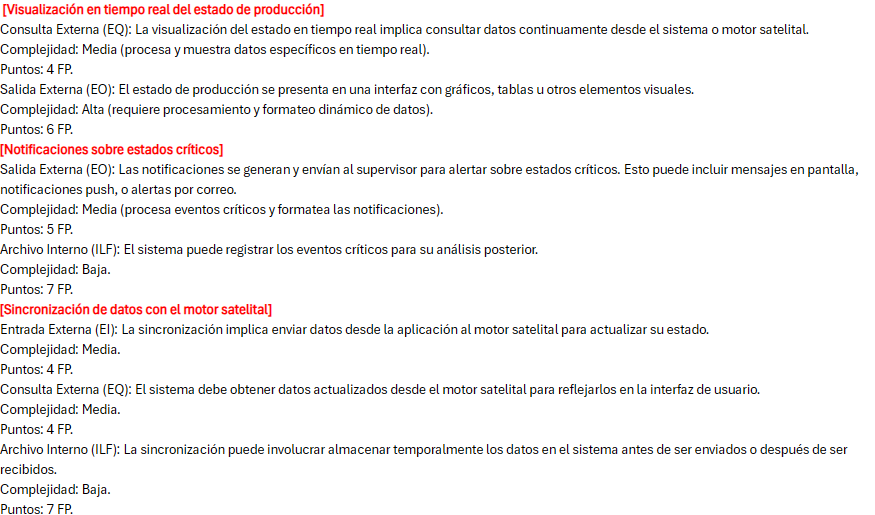
\includegraphics[width=1.0\textwidth]
		{Imagenes/PathAyuda/FpsComunicacionPiso.png}
		\caption{Puntos de Función - Comunicación con el Control de Piso 
		}\label{a2}
	\end{figure}
	
	\begin{figure}[H]
		\centering
		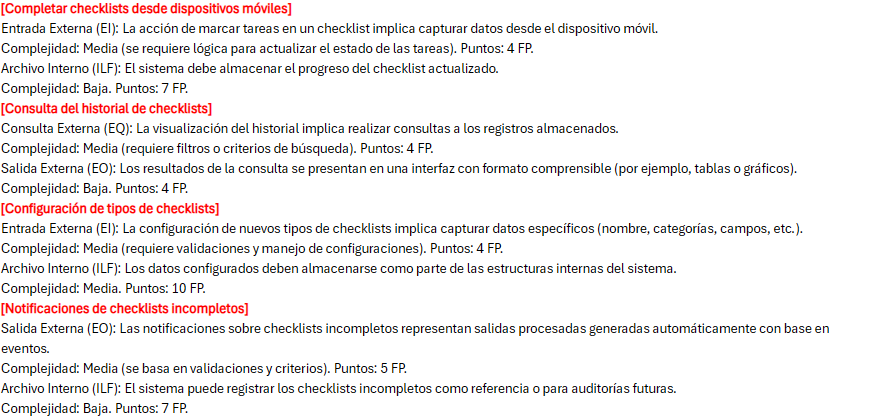
\includegraphics[width=1.0\textwidth]
		{Imagenes/PathAyuda/FpsChecklistsInteractivos.png}
		\caption{Puntos de Función - Gestión de Checklists Interactivos 
		}\label{a2}
	\end{figure}
	
	\begin{figure}[H]
		\centering
		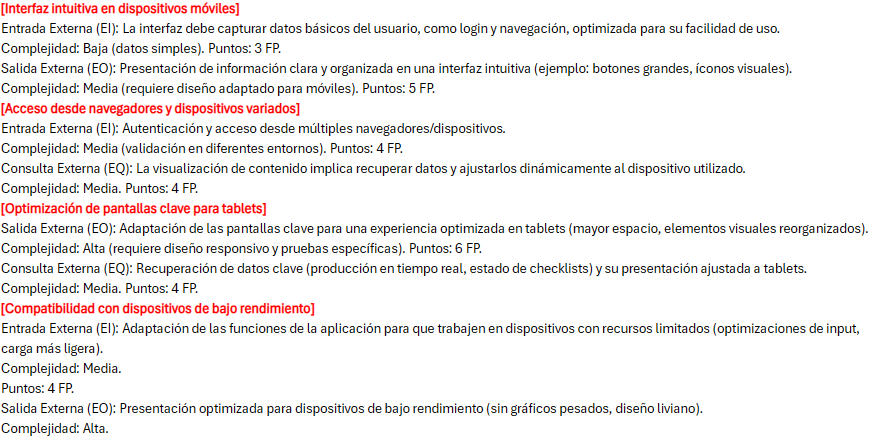
\includegraphics[width=1.0\textwidth]
		{Imagenes/PathAyuda/FpsInterfacesUsuario.png}
		\caption{Puntos de Función - Desarrollo de Interfaces de Usuario Adaptativas 
		}\label{a2}
	\end{figure}
	
	\begin{figure}[H]
		\centering
		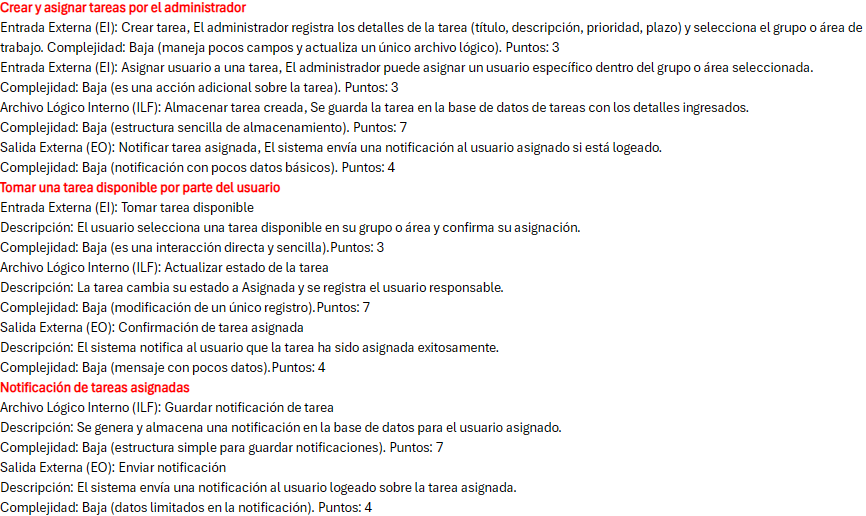
\includegraphics[width=1.0\textwidth]
		{Imagenes/PathAyuda/FpsTaskmanager.png}
		\caption{Puntos de Función - Task manager 
		}\label{a2}
	\end{figure}
	
	\begin{figure}[H]
		\centering
		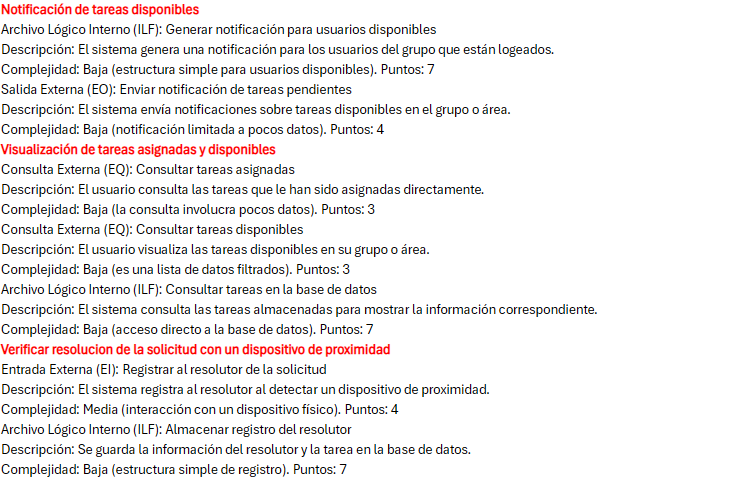
\includegraphics[width=1.0\textwidth]
		{Imagenes/PathAyuda/FpsTaskmanager2.png}
		\caption{Puntos de Función - Task manager 
		}\label{a2}
	\end{figure}
	
	\begin{figure}[H]
		\centering
		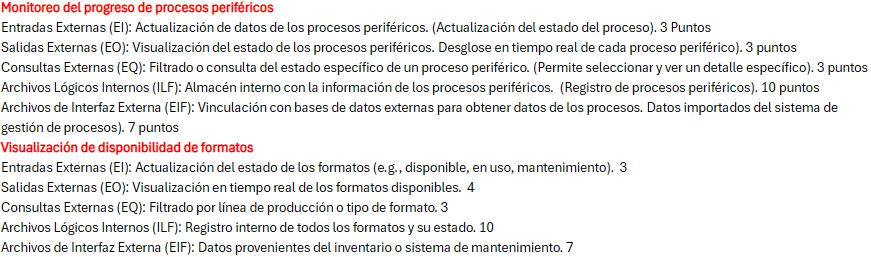
\includegraphics[width=1.0\textwidth]
		{Imagenes/PathAyuda/FpsSMED.png}
		\caption{Puntos de Función - SMED
		}\label{a2}
	\end{figure}
	
	\begin{figure}[H]
		\centering
		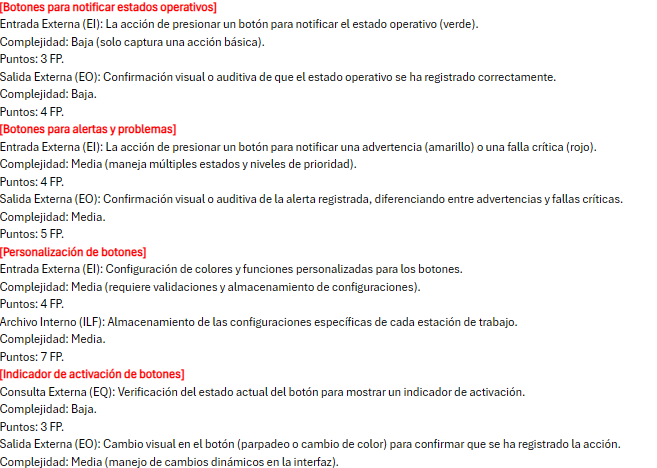
\includegraphics[width=1.0\textwidth]
		{Imagenes/PathAyuda/FpsBotonesANDON.png}
		\caption{Puntos de Función - Simulación de Botones del Sistema ANDON 
		}\label{a2}
	\end{figure}

	
	\begin{figure}[H]
		\centering
		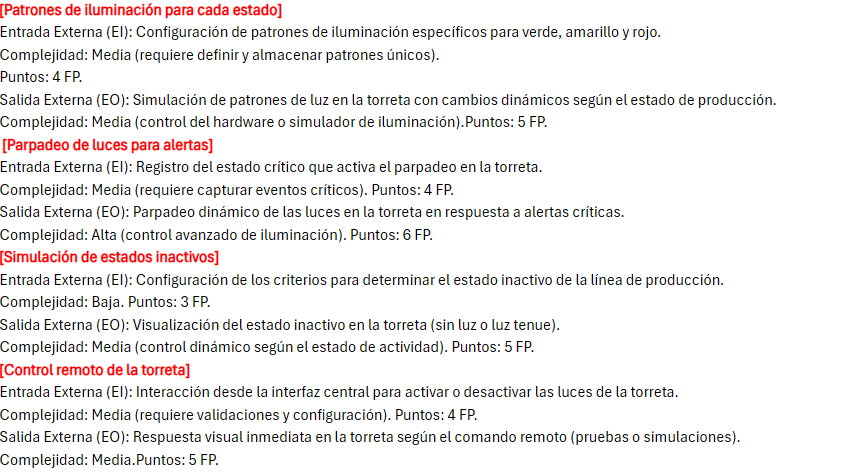
\includegraphics[width=1.0\textwidth]
		{Imagenes/PathAyuda/FpsTorretasLuminosas.png}
		\caption{Puntos de Función - Configuración y Simulación de Torretas Luminosas  
		}\label{a2}
	\end{figure}
	
	\begin{figure}[H]
		\centering
		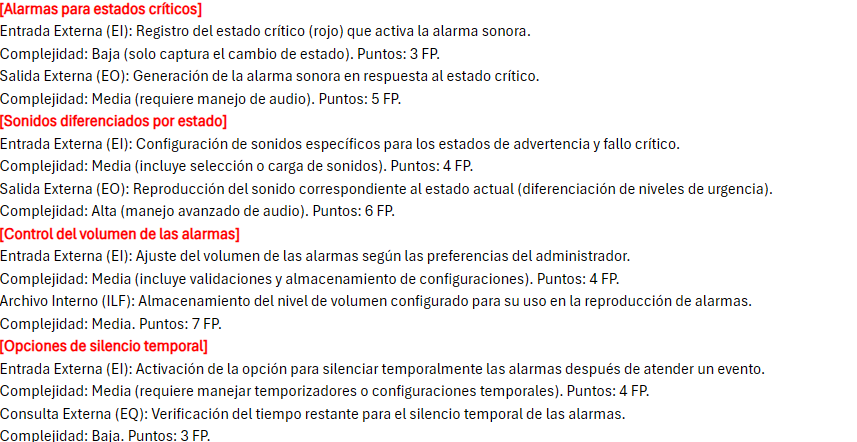
\includegraphics[width=1.0\textwidth]
		{Imagenes/PathAyuda/FpsAlarmasNotifiaciones.png}
		\caption{Puntos de Función - Implementación de Alarmas y Notificaciones Auditivas 
		}\label{a2}
	\end{figure}
	
	\begin{figure}[H]
		\centering
		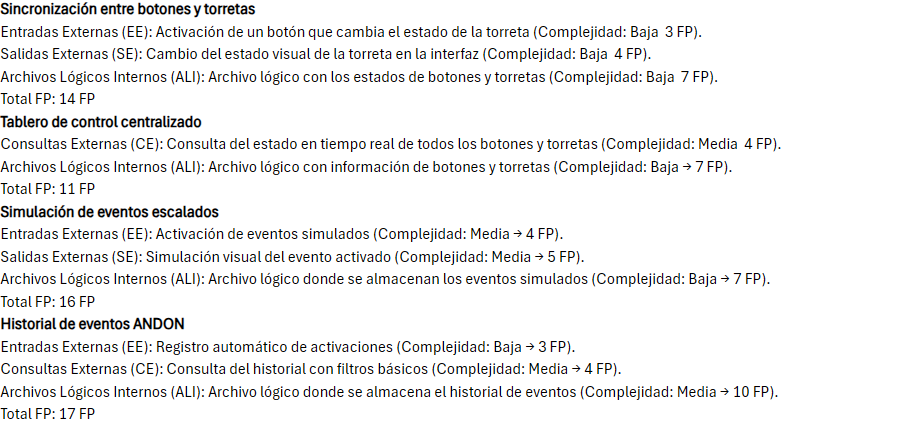
\includegraphics[width=1.0\textwidth]
		{Imagenes/PathAyuda/FpsSimulacion.png}
		\caption{Puntos de Función - Integración y Simulación de la Interfaz ANDON Completa 
		}\label{a2}
	\end{figure}
	
	\begin{figure}[H]
		\centering
		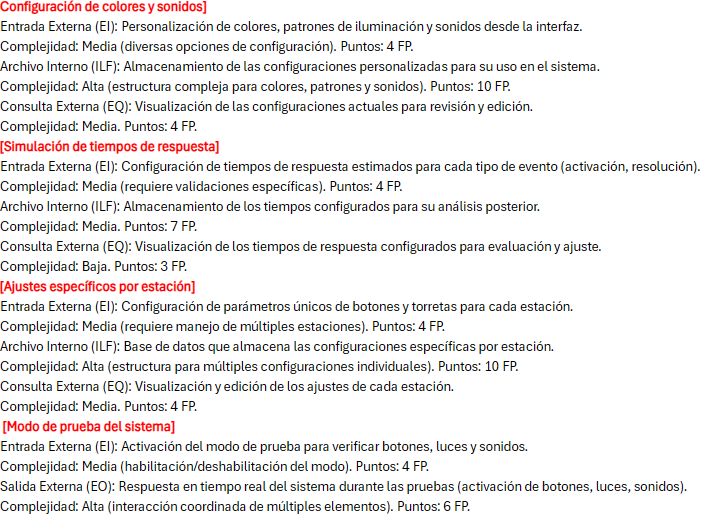
\includegraphics[width=1.0\textwidth]
		{Imagenes/PathAyuda/FpsPersonalizacionAndon.png}
		\caption{Puntos de Función - Personalización y Configuración del Sistema ANDON
		}\label{a2}
	\end{figure}
	
	\begin{figure}[H]
		\centering
		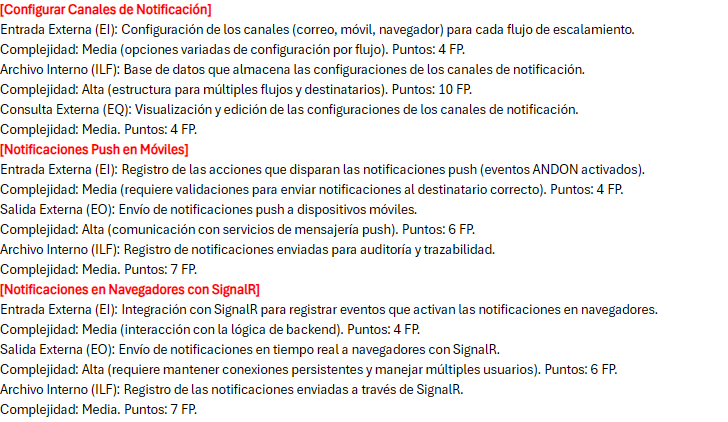
\includegraphics[width=1.0\textwidth]
		{Imagenes/PathAyuda/FpsMultiCanal.png}
		\caption{Puntos de Función - Integración de Notificaciones Multi-Canal
		}\label{a2}
	\end{figure}
	
	\begin{figure}[H]
		\centering
		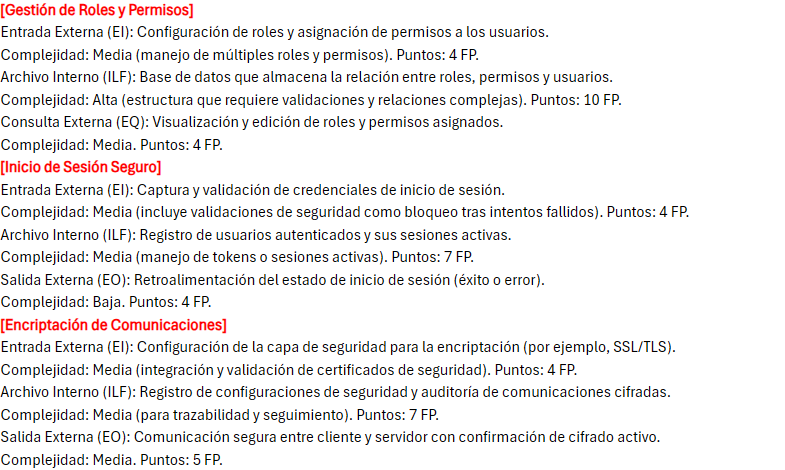
\includegraphics[width=1.0\textwidth]
		{Imagenes/PathAyuda/FpsSeguridadAutenticacion.png}
		\caption{Puntos de Función - Seguridad y Autenticación
		}\label{a2}
	\end{figure}
	
	\begin{figure}[H]
		\centering
		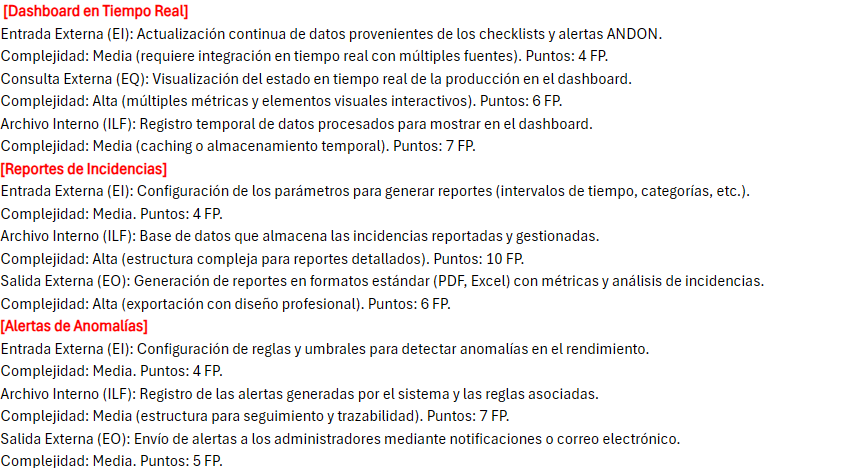
\includegraphics[width=1.0\textwidth]
		{Imagenes/PathAyuda/FpsMonitoreoReportes.png}
		\caption{Puntos de Función - Monitoreo y Reportes
		}\label{a2}
	\end{figure}
	
	\begin{figure}[H]
		\centering
		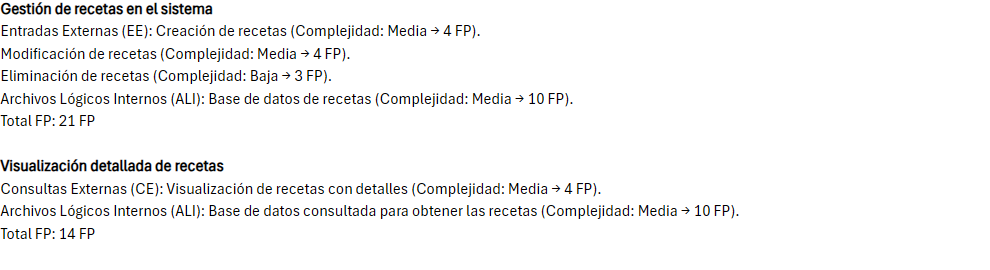
\includegraphics[width=1.0\textwidth]
		{Imagenes/PathAyuda/FpsRecetas.png}
		\caption{Puntos de Función - Recetas
		}\label{a2}
	\end{figure}
	
	\begin{figure}[H]
		\centering
		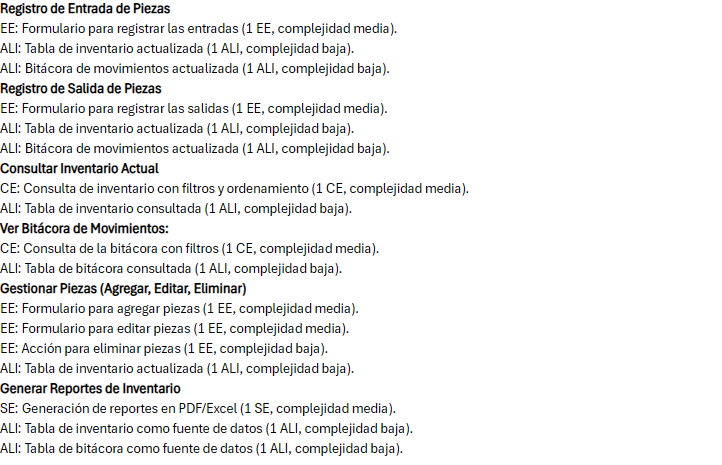
\includegraphics[width=1.0\textwidth]
		{Imagenes/PathAyuda/FpsInventarios.png}
		\caption{Puntos de Función - Inventarios
		}\label{a2}
	\end{figure}
	
	\begin{figure}[H]
		\centering
		\includegraphics[width=1.0\textwidth]
		{Imagenes/PathAyuda/FpsProgramaciónTareas.png}
		\caption{Puntos de Función - Programación de tareas 
		}\label{a2}
	\end{figure}
\newpage

\subsection{Casos de prueba}

	Como parte del proceso de aseguramiento de calidad para el sistema Path de Ayuda, se elaboró un documento estructurado de casos de prueba, organizados por épicas y sus respectivos casos de prueba.\\
	
	El propósito principal de este documento fue definir y estructurar pruebas que permitieran evaluar el cumplimiento de los requerimientos antes de la fase de desarrollo, asegurando que el sistema funcione correctamente bajo diferentes condiciones.\\
	
	El documento de casos de prueba se organizó por épicas, y dentro de cada épica se definieron los escenarios a evaluar.\\
	
	{\leftskip=1em 
	\noindent 
		\textbf{Escenario:} Situación específica en la que se ejecutará la prueba.
	\par}
	
	{\leftskip=1em 
	\noindent 
		\textbf{Prerrequisitos:} Condiciones que deben cumplirse antes de ejecutar la prueba
	\par}

	{\leftskip=1em 
	\noindent 
		\textbf{Datos de Entrada:} Información que se ingresará en el sistema para la ejecución de la prueba.
	\par}

	{\leftskip=1em 
	\noindent 
		\textbf{Resultados Esperados:} Comportamiento esperado del sistema tras ejecutar la prueba.
	\par}

	{\leftskip=1em 
	\noindent 
		\textbf{Escenarios Positivos:} Pruebas en las que el sistema responde correctamente según lo esperado.
	\par}

	{\leftskip=1em 
	\noindent 
		\textbf{Escenarios Negativos:} Pruebas en las que se validan errores o respuestas incorrectas del sistema.\\
	\par}
	
	\begin{figure}[H]
		\centering
		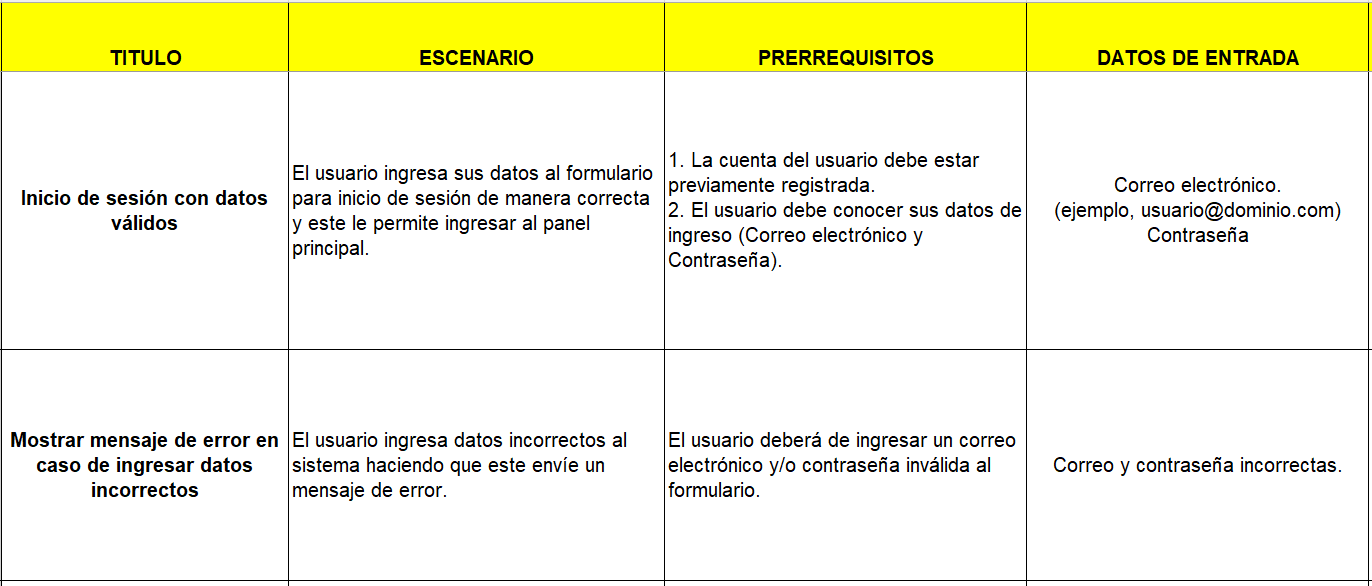
\includegraphics[width=1.0\textwidth]
		{Imagenes/PathAyuda/CPLogin.png}
		\caption{Caso de Prueba - Log-in 
		}\label{a2}
	\end{figure}
	
	\begin{figure}[H]
		\centering
		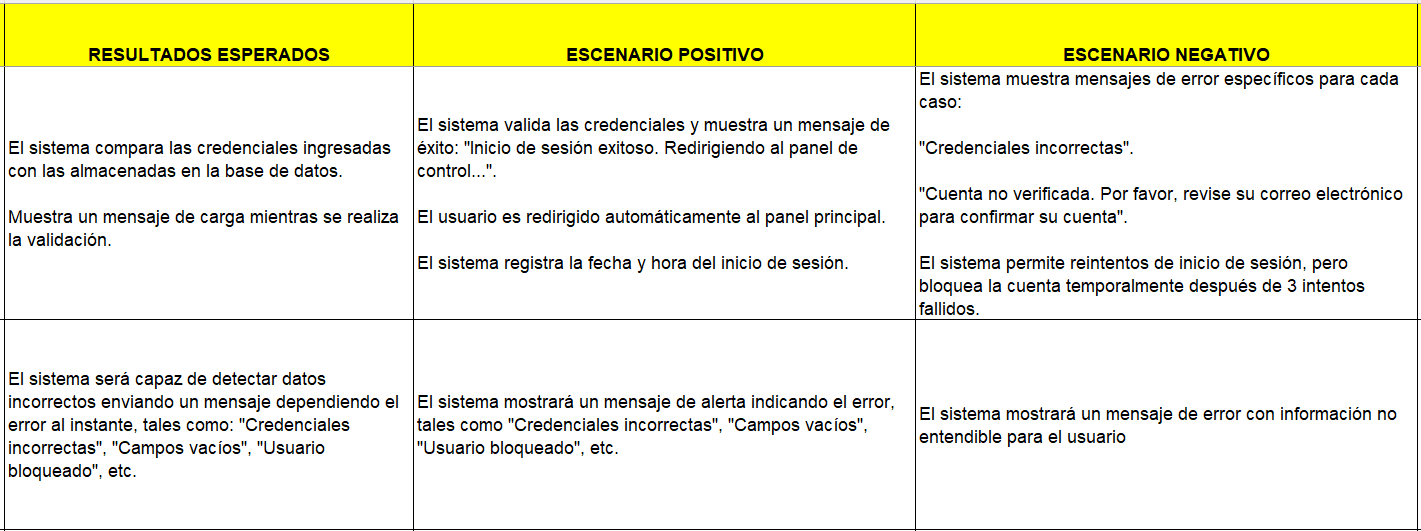
\includegraphics[width=1.0\textwidth]
		{Imagenes/PathAyuda/CPLogin2.png}
		\caption{Caso de Prueba - Log-in 
		}\label{a2}
	\end{figure}

	\begin{figure}[H]
		\centering
		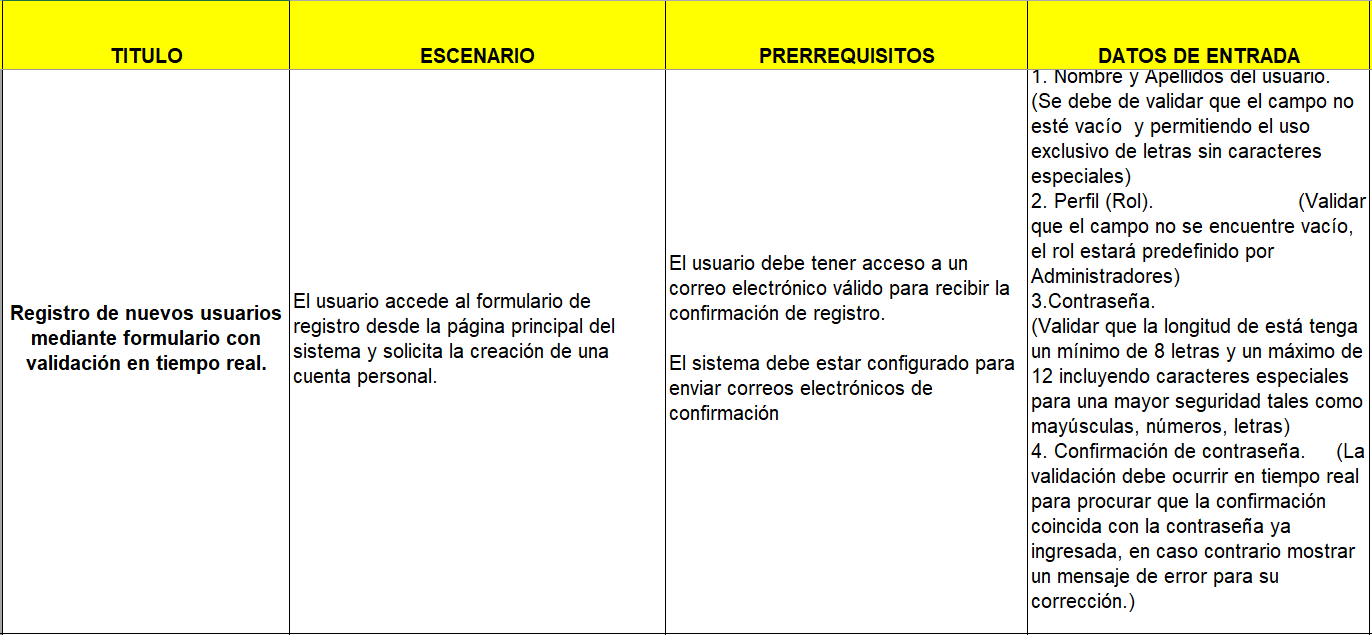
\includegraphics[width=1.0\textwidth]
		{Imagenes/PathAyuda/CPRegistroUsuario.png}
		\caption{Caso de Prueba - Registro de Usuario 
		}\label{a2}
	\end{figure}
	
	\begin{figure}[H]
		\centering
		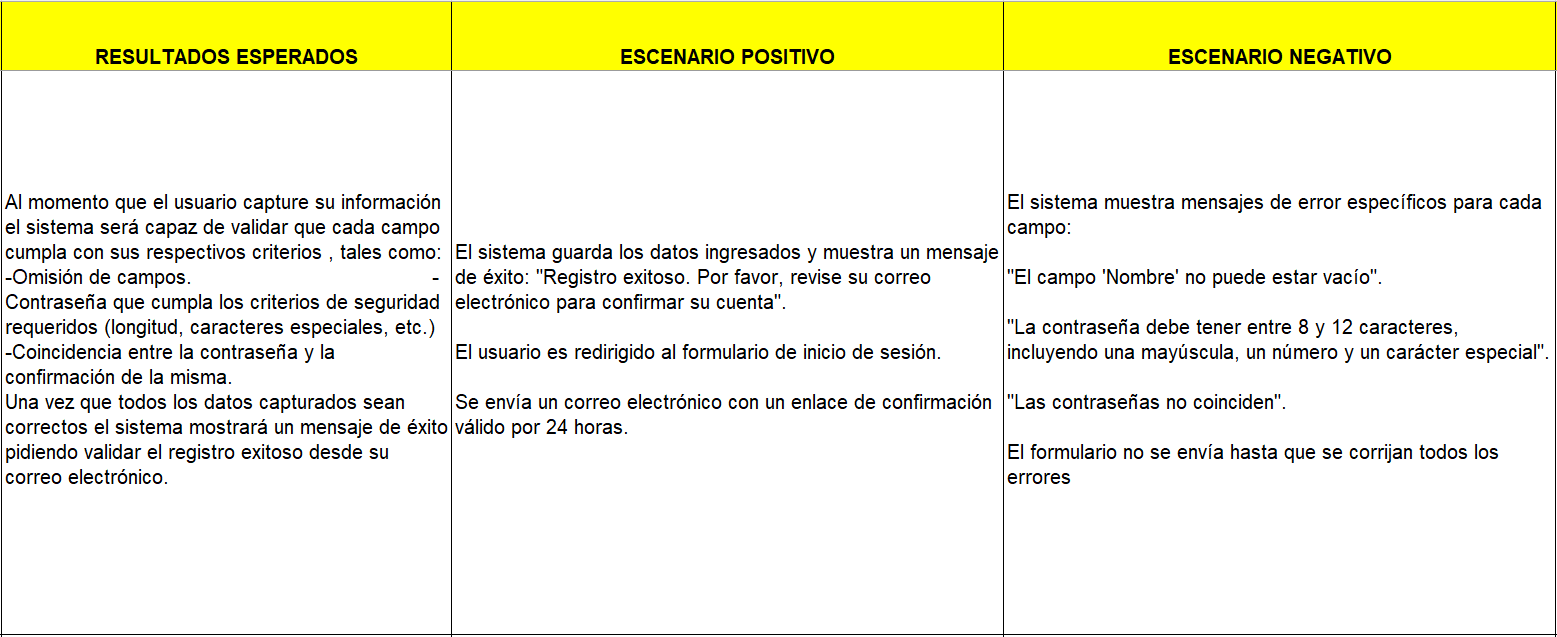
\includegraphics[width=1.0\textwidth]
		{Imagenes/PathAyuda/CPRegistroUsuario2.png}
		\caption{Caso de Prueba - Registro de Usuario
		}\label{a2}
	\end{figure}
	
	\begin{figure}[H]
		\centering
		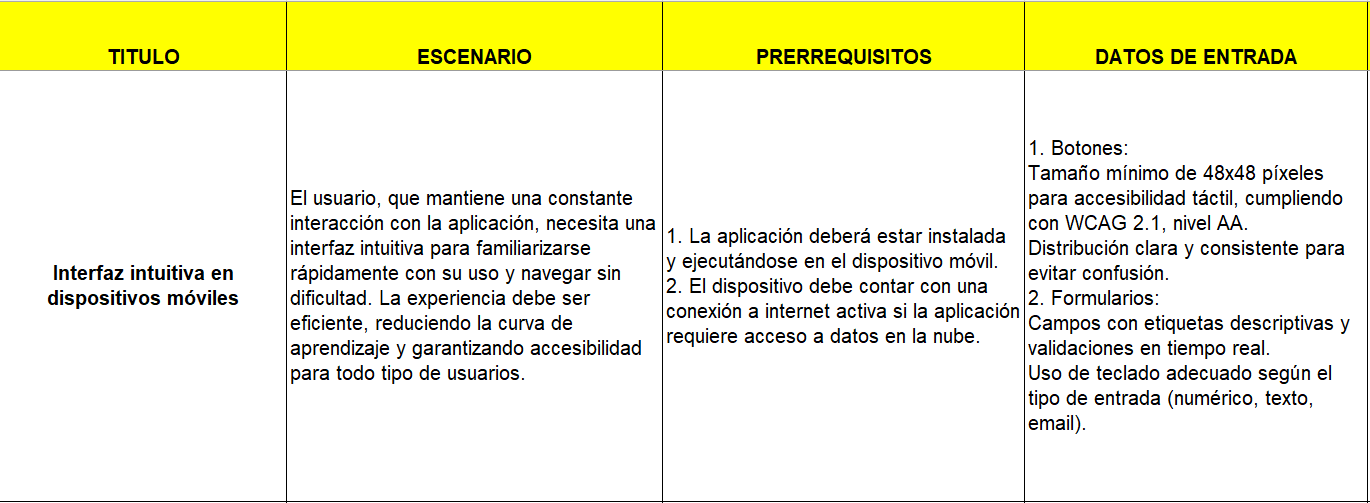
\includegraphics[width=1.0\textwidth]
		{Imagenes/PathAyuda/CPInterfaces.png}
		\caption{Caso de Prueba - Desarrollo de Interfaces de Usuario Adaptativas 
		}\label{a2}
	\end{figure}
	
	\begin{figure}[H]
		\centering
		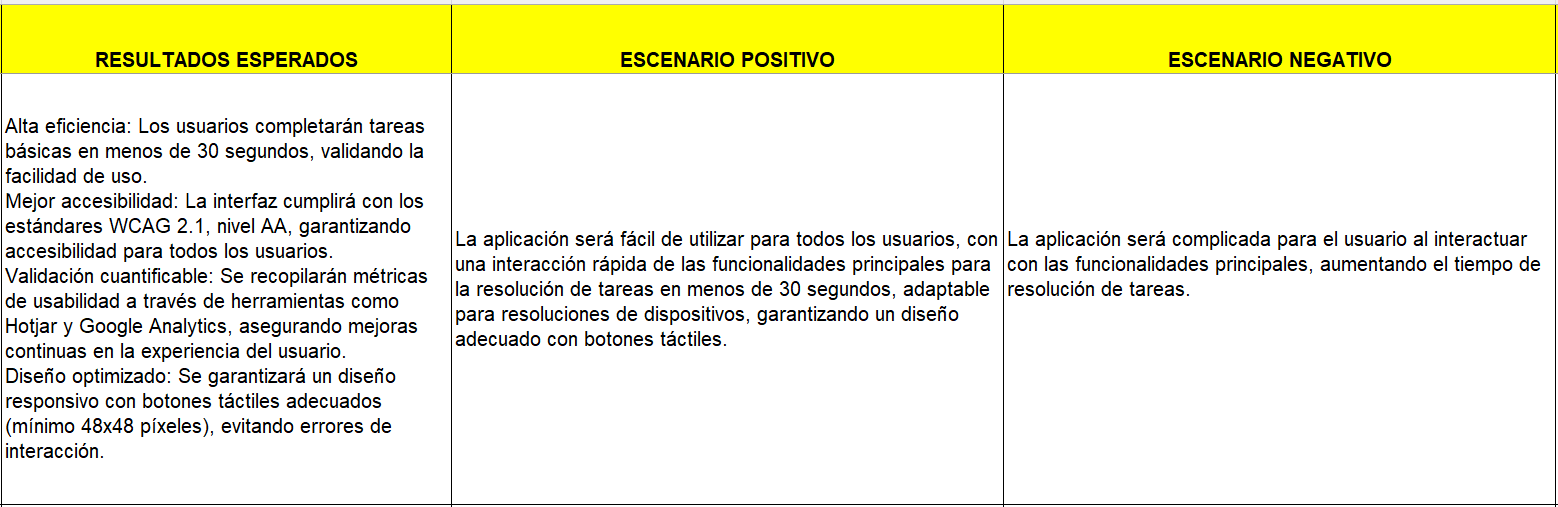
\includegraphics[width=1.0\textwidth]
		{Imagenes/PathAyuda/CPInterfaces2.png}
		\caption{Caso de Prueba - Desarrollo de Interfaces de Usuario Adaptativas
		}\label{a2}
	\end{figure}
	
	\begin{figure}[H]
		\centering
		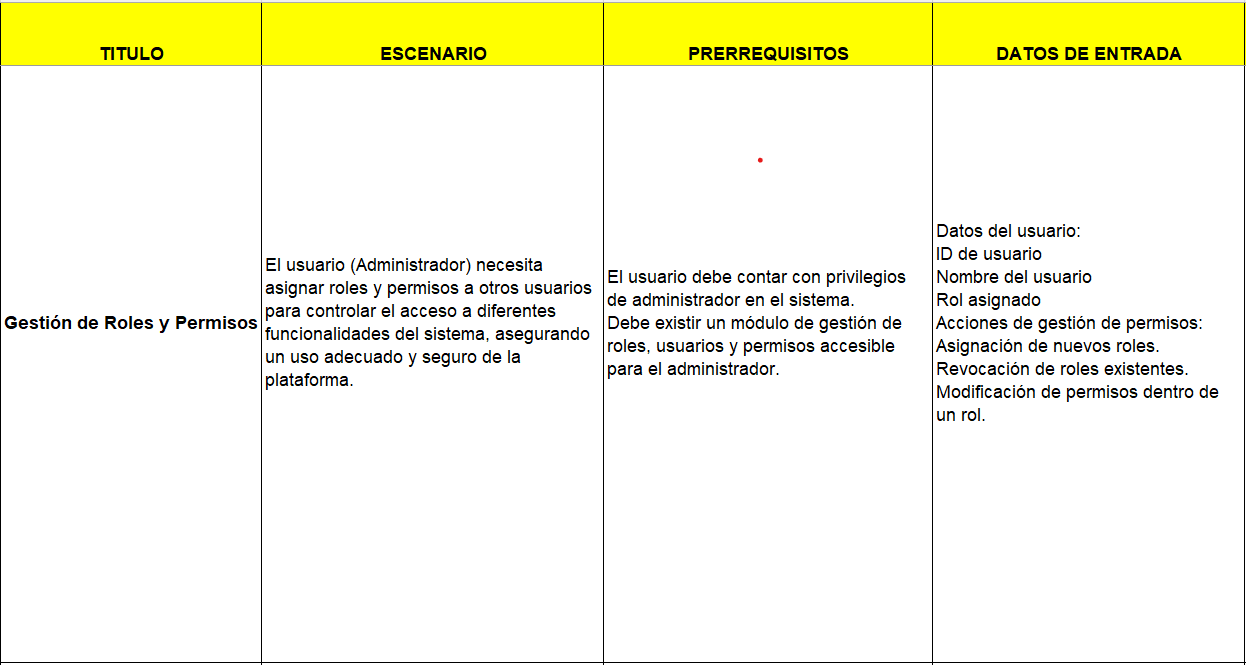
\includegraphics[width=1.0\textwidth]
		{Imagenes/PathAyuda/CPSeguridadAutenticacion.png}
		\caption{Caso de Prueba - Seguridad y  Autenticación
		}\label{a2}
	\end{figure}
	
	\begin{figure}[H]
		\centering
		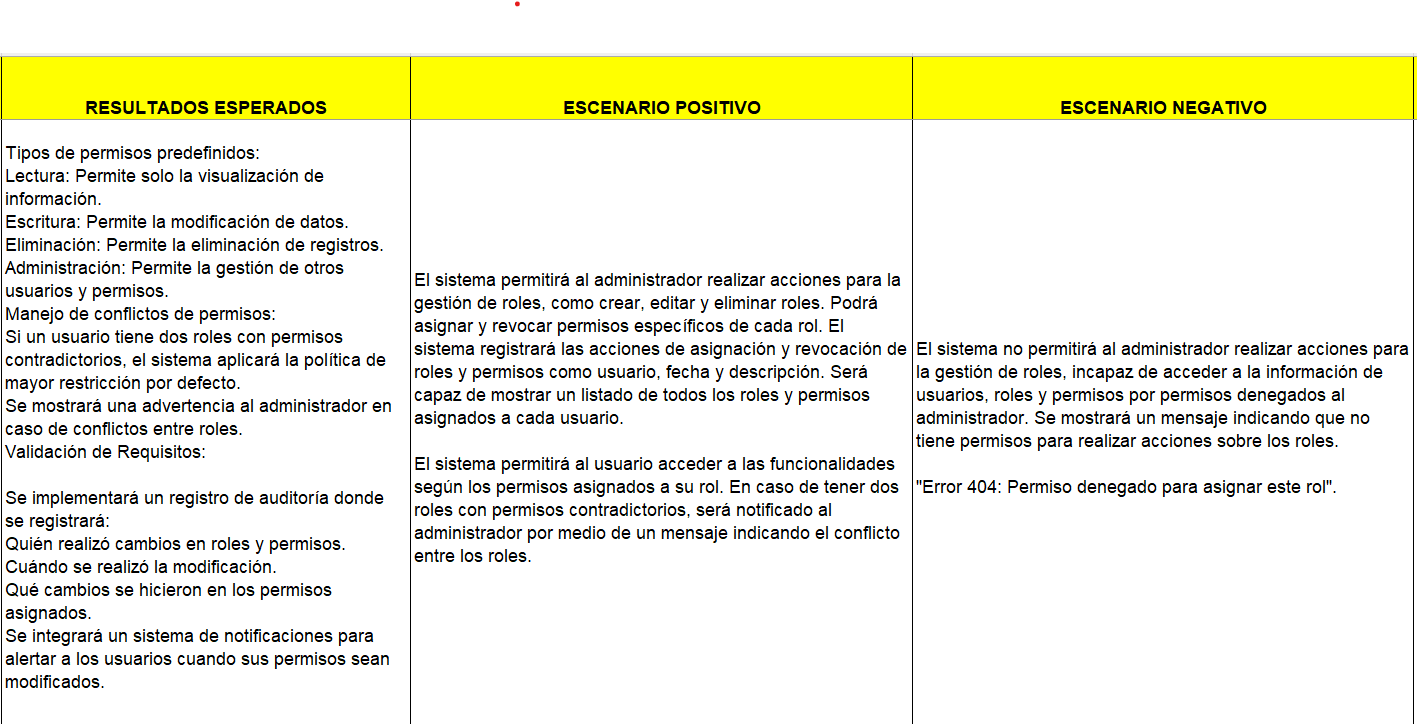
\includegraphics[width=1.0\textwidth]
		{Imagenes/PathAyuda/CPSeguridadAutenticacion2.png}
		\caption{Caso de Prueba - Seguridad y  Autenticación
		}\label{a2}
	\end{figure}
	
	\begin{figure}[H]
		\centering
		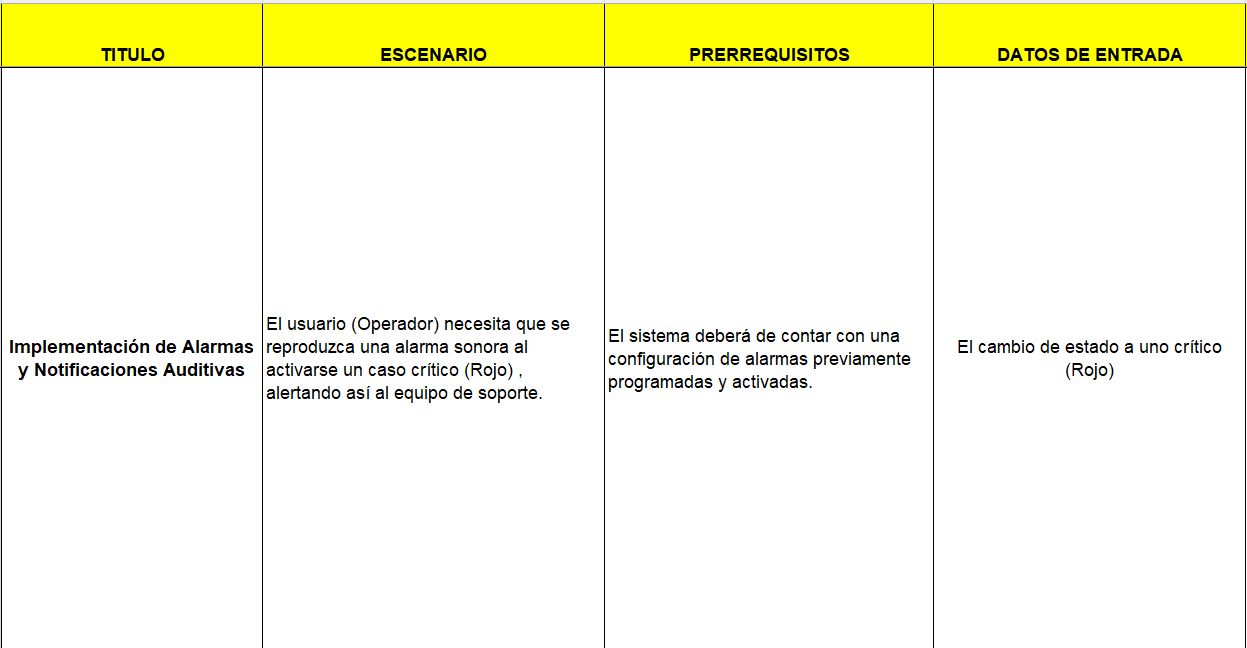
\includegraphics[width=1.0\textwidth]
		{Imagenes/PathAyuda/CPPathAyuda.png}
		\caption{Caso de Prueba - Path de ayuda /  ANDON
		}\label{a2}
	\end{figure}
	
	\begin{figure}[H]
		\centering
		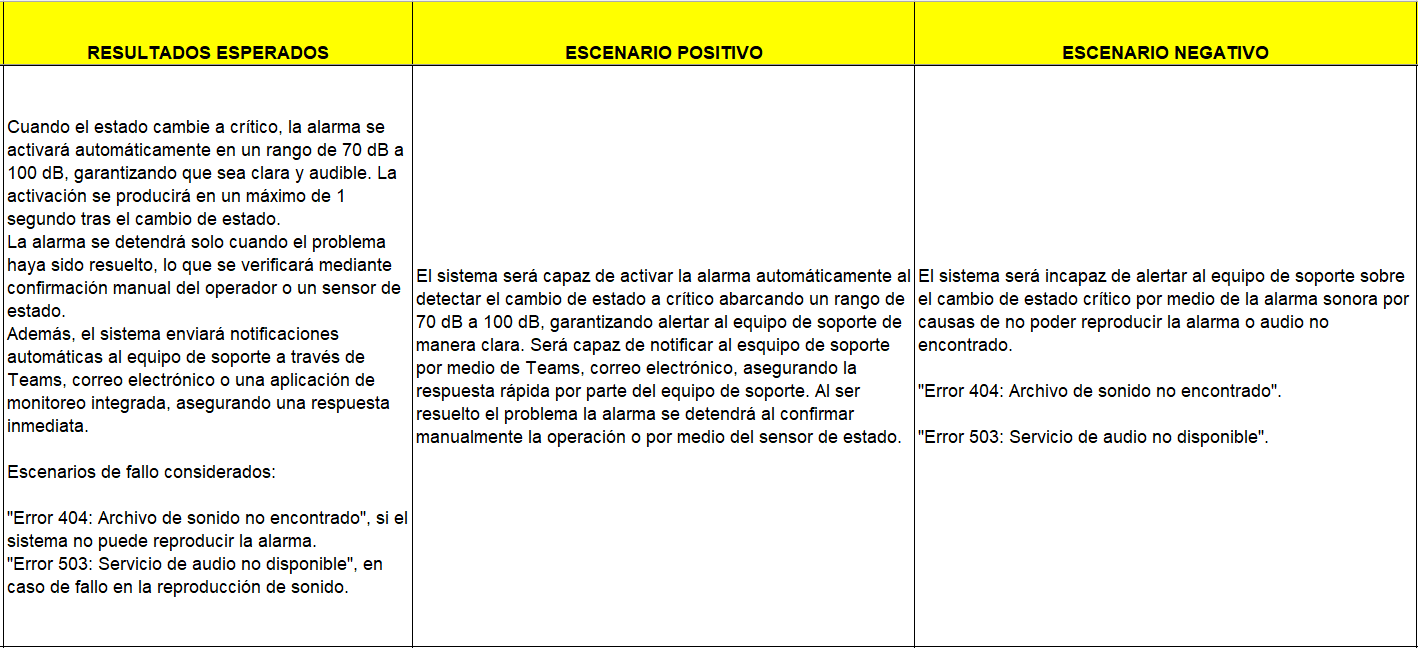
\includegraphics[width=1.0\textwidth]
		{Imagenes/PathAyuda/CPPathAyuda2.png}
		\caption{Caso de Prueba - Path de ayuda /  ANDON
		}\label{a2}
	\end{figure}
	
	\begin{figure}[H]
		\centering
		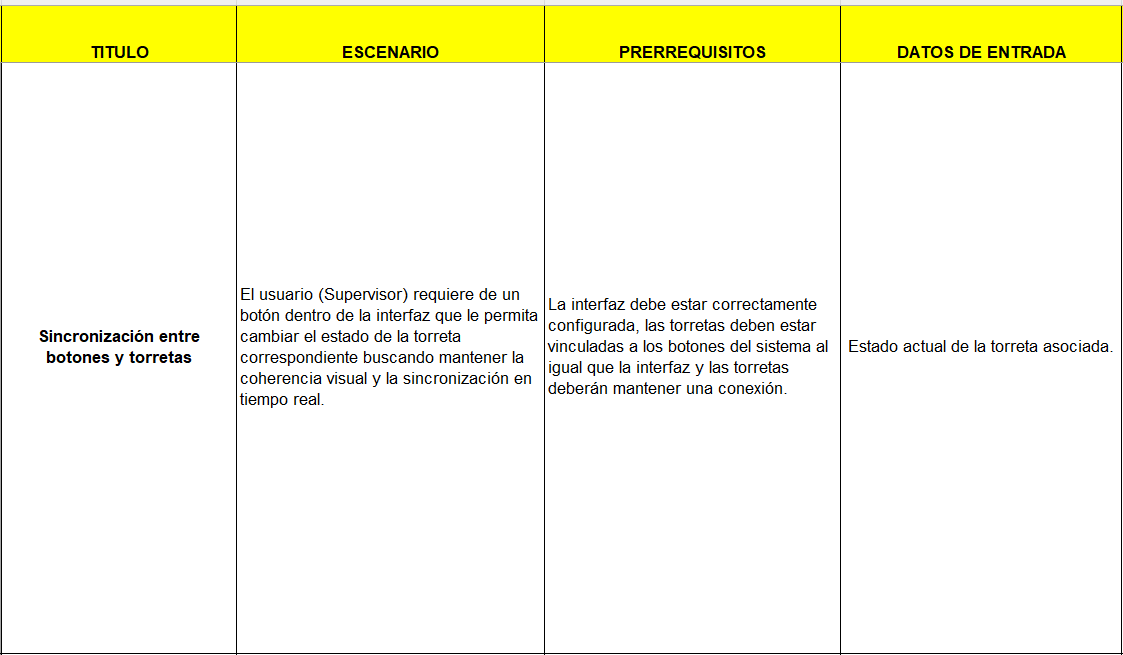
\includegraphics[width=1.0\textwidth]
		{Imagenes/PathAyuda/CPANDON.png}
		\caption{Caso de Prueba - Integración y simulación - ANDON
		}\label{a2}
	\end{figure}
	
	\begin{figure}[H]
		\centering
		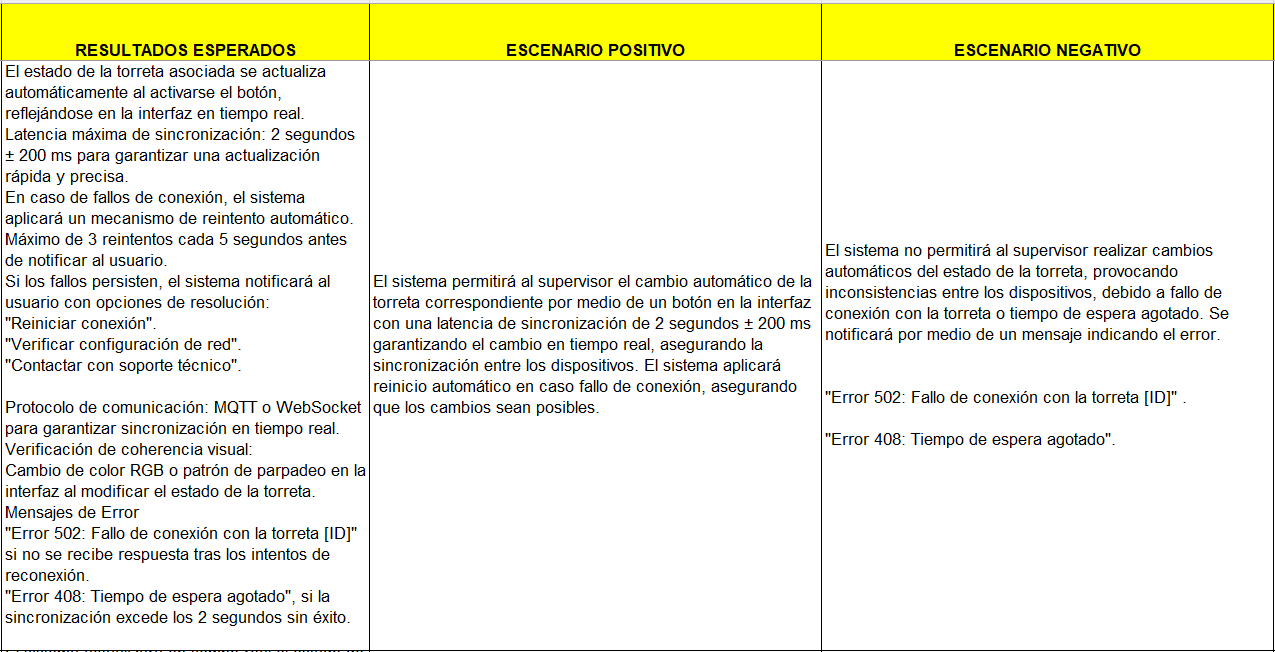
\includegraphics[width=1.0\textwidth]
		{Imagenes/PathAyuda/CPANDON2.png}
		\caption{Caso de Prueba - Integración y simulación - ANDON
		}\label{a2}
	\end{figure}
	
	\begin{figure}[H]
		\centering
		\includegraphics[width=1.0\textwidth]
		{Imagenes/PathAyuda/CPPesonalizaciónANDON.png}
		\caption{Caso de Prueba - Personalización y configuración - ANDON 
		}\label{a2}
	\end{figure}
	
	\begin{figure}[H]
		\centering
		\includegraphics[width=1.0\textwidth]
		{Imagenes/PathAyuda/CPPesonalizaciónANDON2.png}
		\caption{Caso de Prueba - Personalización y configuración - ANDON
		}\label{a2}
	\end{figure}
	
	\begin{figure}[H]
		\centering
		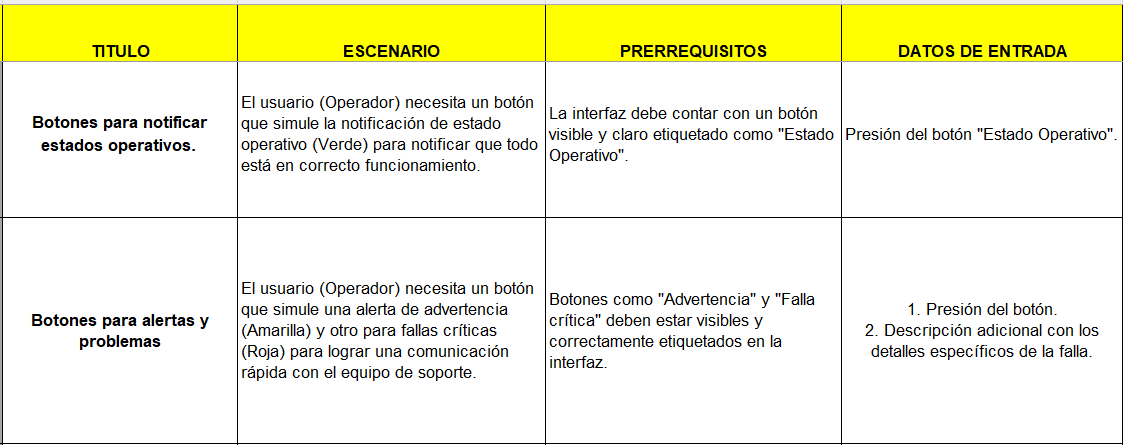
\includegraphics[width=1.0\textwidth]
		{Imagenes/PathAyuda/CPBotonesAndon.png}
		\caption{Caso de Prueba - Simulación de botones - ANDON
		}\label{a2}
	\end{figure}
	
	\begin{figure}[H]
		\centering
		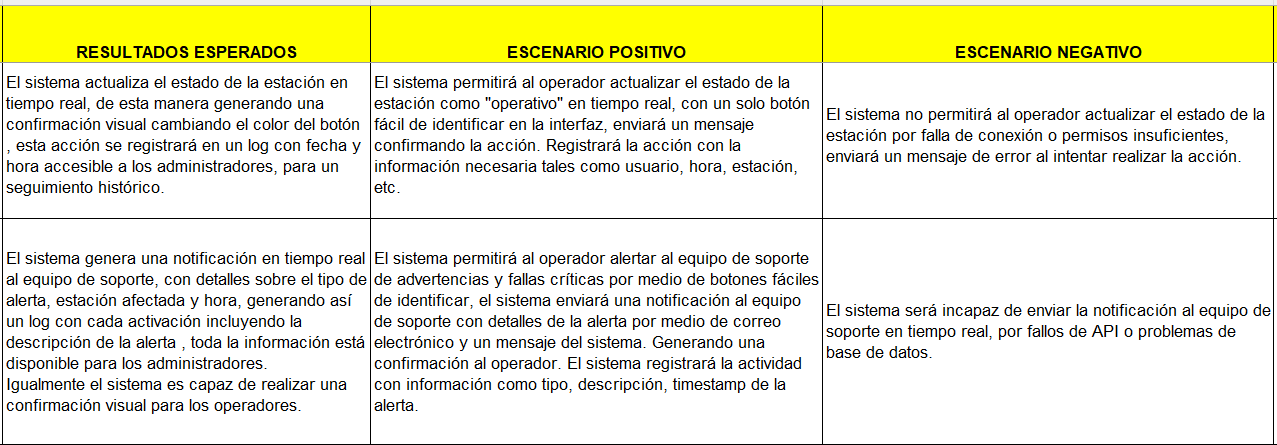
\includegraphics[width=1.0\textwidth]
		{Imagenes/PathAyuda/CPBotonesAndon2.png}
		\caption{Caso de Prueba - Simulación de botones - ANDON
		}\label{a2}
	\end{figure}
	
	\begin{figure}[H]
		\centering
		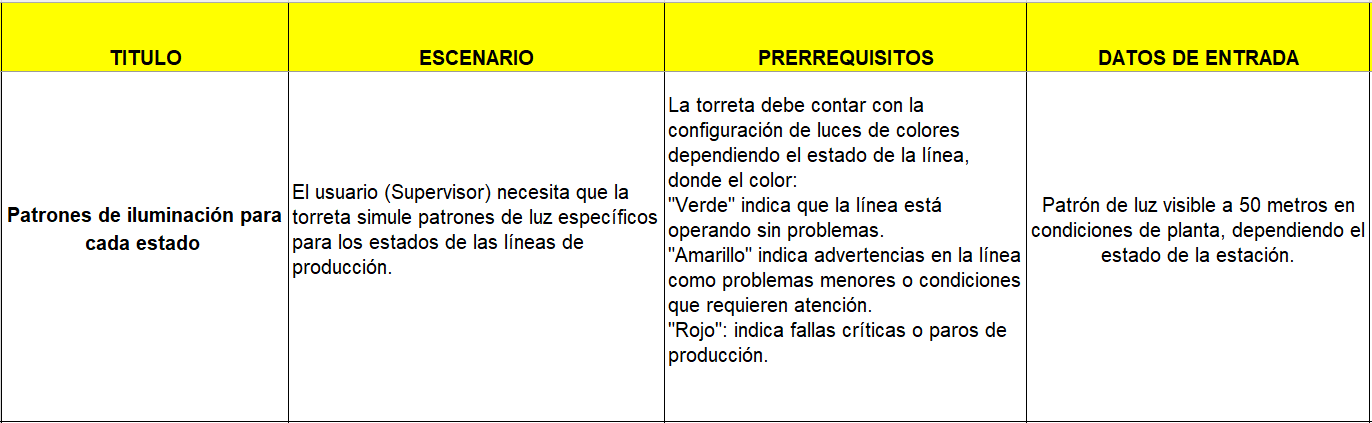
\includegraphics[width=1.0\textwidth]
		{Imagenes/PathAyuda/CPTorreta.png}
		\caption{Caso de Prueba - Configuración y Simulación de Torreta Luminosa
		}\label{a2}
	\end{figure}
	
	\begin{figure}[H]
		\centering
		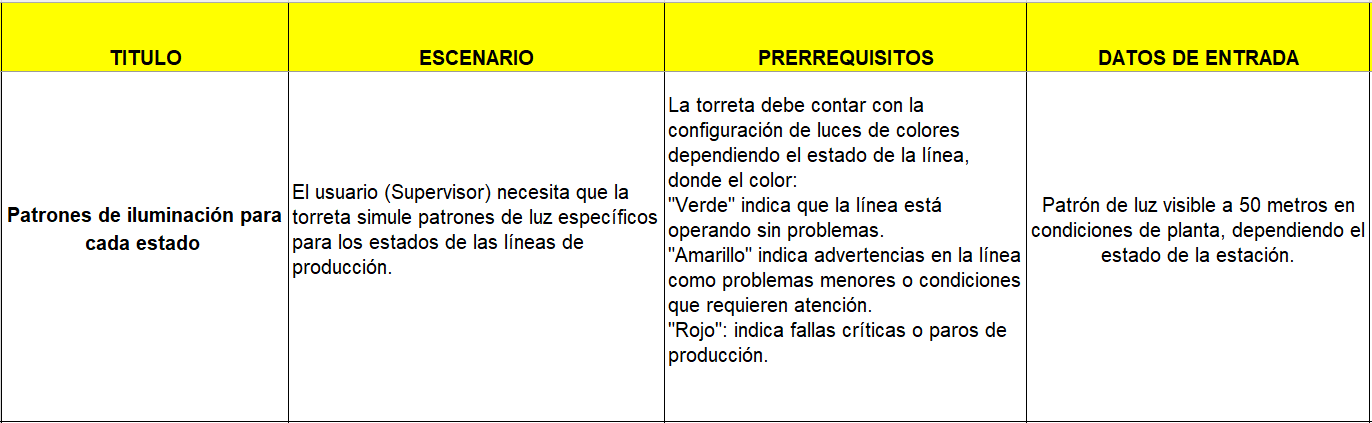
\includegraphics[width=1.0\textwidth]
		{Imagenes/PathAyuda/CPTorreta.png}
		\caption{Caso de Prueba - Configuración y Simulación de Torreta Luminosa
		}\label{a2}
	\end{figure}
	
	\begin{figure}[H]
		\centering
		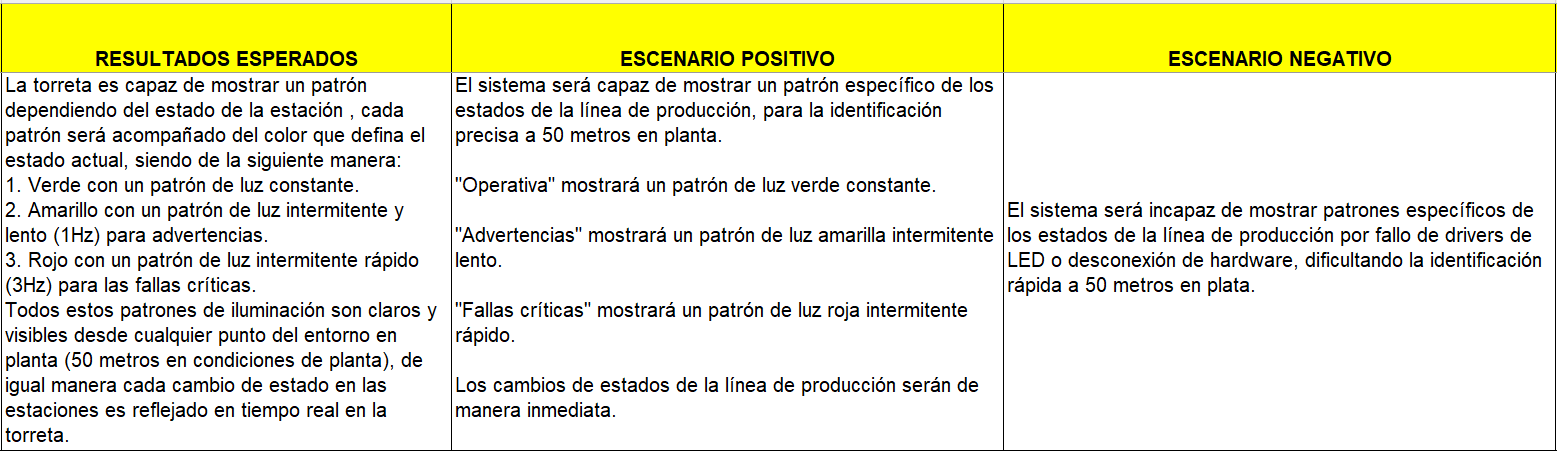
\includegraphics[width=1.0\textwidth]
		{Imagenes/PathAyuda/CPTorreta2.png}
		\caption{Caso de Prueba - Configuración y Simulación de Torreta Luminosa
		}\label{a2}
	\end{figure}
	
	\begin{figure}[H]
		\centering
		\includegraphics[width=1.0\textwidth]
		{Imagenes/PathAyuda/CPMultiCanal.png}
		\caption{Caso de Prueba - Notificaciones Multi-Canal
		}\label{a2}
	\end{figure}
	
	\begin{figure}[H]
		\centering
		\includegraphics[width=1.0\textwidth]
		{Imagenes/PathAyuda/CPMultiCanal2.png}
		\caption{Caso de Prueba - Notificaciones Multi-Canal
		}\label{a2}
	\end{figure}
	
	\begin{figure}[H]
		\centering
		\includegraphics[width=1.0\textwidth]
		{Imagenes/PathAyuda/CPSMED.png}
		\caption{Caso de Prueba - SMED
		}\label{a2}
	\end{figure}
	
	\begin{figure}[H]
		\centering
		\includegraphics[width=1.0\textwidth]
		{Imagenes/PathAyuda/CPSMED2.png}
		\caption{Caso de Prueba - SMED
		}\label{a2}
	\end{figure}
	
	\begin{figure}[H]
		\centering
		\includegraphics[width=0.9\textwidth]
		{Imagenes/PathAyuda/CPRecetas.png}
		\caption{Caso de Prueba - Gestión de Recetas
		}\label{a2}
	\end{figure}
	
	\begin{figure}[H]
		\centering
		\includegraphics[width=1.0\textwidth]
		{Imagenes/PathAyuda/CPRecetas2.png}
		\caption{Caso de Prueba - Gestión de Recetas
		}\label{a2}
	\end{figure}
	
	\begin{figure}[H]
		\centering
		\includegraphics[width=1.0\textwidth]
		{Imagenes/PathAyuda/CPLineaProduccion.png}
		\caption{Caso de Prueba - Trafico de Líneas de Producción
		}\label{a2}
	\end{figure}
	
	\begin{figure}[H]
		\centering
		\includegraphics[width=1.0\textwidth]
		{Imagenes/PathAyuda/CPLineaProduccion2.png}
		\caption{Caso de Prueba - Trafico de Líneas de Producción
		}\label{a2}
	\end{figure}
	
	\begin{figure}[H]
		\centering
		\includegraphics[width=1.0\textwidth]
		{Imagenes/PathAyuda/CPTask.png}
		\caption{Caso de Prueba - Task Manager (Incidencias ANDON)
		}\label{a2}
	\end{figure}
	
	\begin{figure}[H]
		\centering
		\includegraphics[width=1.0\textwidth]
		{Imagenes/PathAyuda/CPTask2.png}
		\caption{Caso de Prueba - Task Manager (Incidencias ANDON)
		}\label{a2}
	\end{figure}
	
	\newpage
	

\section{Calculadora Nutricional}

	El proyecto Calculadora Nutricional tiene como objetivo modernizar una herramienta desarrollada en 2011 para el cálculo de nutrición parenteral en pacientes adultos, trasladándola a una plataforma web accesible y funcional. La versión original, distribuida en discos físicos y operada mediante un programa instalable, quedó obsoleta con el tiempo, limitando su uso y dificultando la promoción de mezclas individualizadas.\\
	
	Para garantizar un desarrollo estructurado y eficiente, se llevó a cabo una documentación completa del proyecto. Este trabajo permitió establecer una base sólida para la planificación y ejecución del desarrollo, asegurando que cada aspecto del sistema estuviera bien definido antes de su implementación.\\
	
	Gracias a esta documentación, se logró una mejor organización del proyecto, facilitando la identificación de necesidades y asegurando que las funcionalidades estuvieran alineadas con los objetivos planteados.Además, permitió estructurar de manera clara las mejoras con respecto a la versión anterior, optimizando el desarrollo y asegurando que la herramienta final sea eficiente, accesible y alineada con las necesidades del sector salud.

\subsection{Levantamiento de requerimientos}

	Para garantizar que la nueva versión de la Calculadora Nutricional cubriera todas las necesidades del personal de salud y mejorara significativamente la experiencia del usuario, se llevó a cabo un levantamiento de requerimientos detallado. Este proceso permitió identificar limitaciones clave de la versión original y definir nuevas funcionalidades que optimizarían su uso en un entorno web, logrando una herramienta más eficiente, accesible y alineada con las necesidades actuales del sector salud.\\
	
	{\leftskip=1em 
	\noindent 
	\textbf{Usuarios y roles:}\\ 
	Se estableció una diferenciación clara entre usuarios registrados (doctores y personal de salud) y visitantes, asignando permisos personalizados. Esto permitió que los profesionales de la salud pudieran almacenar y recuperar cálculos, mejorando la continuidad en el análisis nutricional.\\
	\par}

	{\leftskip=1em 
	\noindent 
	\textbf{Funcionalidades esenciales:}\\
	Se implementaron características clave como el cálculo de mezclas nutricionales, la impresión de resultados, el almacenamiento de datos en una base de datos segura y una encuesta inicial para recopilar información sobre el uso de la herramienta, permitiendo mejorar su adaptación a los requerimientos.\\
	\par}
	
	{\leftskip=1em 
	\noindent 
	\textbf{Mejoras respecto a la versión anterior:}\\
	Se integraron herramientas de monitoreo avanzadas para conocer quién y desde dónde se utiliza la calculadora, facilitando la toma de decisiones estratégicas en cuanto a promoción, capacitación y mejoras futuras.\\
	\par}
	
	{\leftskip=1em 
	\noindent 
	\textbf{Requisitos técnicos y de usabilidad:}\\
	Se priorizaron aspectos como la accesibilidad, la compatibilidad con dispositivos modernos y una interfaz intuitiva, asegurando que la calculadora fuera fácil de usar y eficiente en distintos contextos clínicos y académicos.\\
	\par}
	

\subsection{Casos de prueba}
	
	Para asegurar la fiabilidad de los cálculos y la correcta implementación de las funcionalidades de la Calculadora Nutricional, se diseñó un conjunto de casos de prueba organizados por épicas y centrados en la precisión de las fórmulas médicas, la gestión de usuarios y la usabilidad del sistema. Cada caso de prueba incluye los elementos clave para su ejecución.\\
	
	

	{\leftskip=1em 
		\noindent 
		\textbf{Escenario:} Situación específica en la que se ejecutará la prueba.
		\par}
	
	{\leftskip=1em 
		\noindent 
		\textbf{Prerrequisitos:} Condiciones que deben cumplirse antes de ejecutar la prueba
		\par}
	
	{\leftskip=1em 
		\noindent 
		\textbf{Datos de Entrada:} Información que se ingresará en el sistema para la ejecución de la prueba.
		\par}
	
	{\leftskip=1em 
		\noindent 
		\textbf{Resultados Esperados:} Comportamiento esperado del sistema tras ejecutar la prueba.
		\par}
	
	{\leftskip=1em 
		\noindent 
		\textbf{Escenarios Positivos:} Pruebas en las que el sistema responde correctamente según lo esperado.
		\par}
	
	{\leftskip=1em 
		\noindent 
		\textbf{Escenarios Negativos:} Pruebas en las que se validan errores o respuestas incorrectas del sistema.\\
		\par}


	Se diseñaron pruebas para garantizar la precisión del sistema, verificando la exactitud de los cálculos, el manejo de errores en los datos de entrada y el acceso adecuado según el tipo de usuario. Además, se validó la correcta generación e impresión de reportes. La documentación detallada de estos casos de prueba permitió establecer un marco sólido para la validación del sistema, asegurando su fiabilidad y facilitando futuras mejoras.\\
	
	
	\begin{figure}[H]
		\centering
		\includegraphics[width=1.0\textwidth]
		{Imagenes/CalculadoraNutricional/CPLogin.png}
		\caption{Caso de Prueba - Log-in
		}\label{a2}
	\end{figure}
	
	\begin{figure}[H]
		\centering
		\includegraphics[width=1.0\textwidth]
		{Imagenes/CalculadoraNutricional/CPLogin2.png}
		\caption{Caso de Prueba - Log-in
		}\label{a2}
	\end{figure}
	
	\begin{figure}[H]
		\centering
		\includegraphics[width=1.0\textwidth]
		{Imagenes/CalculadoraNutricional/CPCuentaMedico.png}
		\caption{Caso de Prueba - Creación de Cuenta para Personal Médico
		}\label{a2}
	\end{figure}
	
	\begin{figure}[H]
		\centering
		\includegraphics[width=1.0\textwidth]
		{Imagenes/CalculadoraNutricional/CPCuentaMedico2.png}
		\caption{Caso de Prueba - Creación de Cuenta para Personal Médico
		}\label{a2}
	\end{figure}
	
	\begin{figure}[H]
		\centering
		\includegraphics[width=1.0\textwidth]
		{Imagenes/CalculadoraNutricional/CPCuentaEstudiante.png}
		\caption{Caso de Prueba - Creación de Cuenta para Personal Médico
		}\label{a2}
	\end{figure}
	
	\begin{figure}[H]
		\centering
		\includegraphics[width=1.0\textwidth]
		{Imagenes/CalculadoraNutricional/CPCuentaEstudiante2.png}
		\caption{Caso de Prueba - Creación de Cuenta para Personal Médico
		}\label{a2}
	\end{figure}
	
	\begin{figure}[H]
		\centering
		\includegraphics[width=1.0\textwidth]
		{Imagenes/CalculadoraNutricional/CPSesionGestion.png}
		\caption{Caso de Prueba - Inicio de Sesión y Gestión de Usuarios
		}\label{a2}
	\end{figure}
	
	\begin{figure}[H]
		\centering
		\includegraphics[width=1.0\textwidth]
		{Imagenes/CalculadoraNutricional/CPSesionGestion2.png}
		\caption{Caso de Prueba - Inicio de Sesión y Gestión de Usuarios
		}\label{a2}
	\end{figure}
	
	
	\begin{figure}[H]
		\centering
		\includegraphics[width=1.0\textwidth]
		{Imagenes/CalculadoraNutricional/CPRolesPermisos.png}
		\caption{Caso de Prueba - Gestión de Roles y Permisos
		}\label{a2}
	\end{figure}
	
	\begin{figure}[H]
		\centering
		\includegraphics[width=1.0\textwidth]
		{Imagenes/CalculadoraNutricional/CPRolesPermisos2.png}
		\caption{Caso de Prueba - Gestión de Roles y Permisos
		}\label{a2}
	\end{figure}
	
	\begin{figure}[H]
		\centering
		\includegraphics[width=1.0\textwidth]
		{Imagenes/CalculadoraNutricional/CPEncuestaEstudiante.png}
		\caption{Caso de Prueba - Encuesta de Registro para Estudiantes y Visitantes
		}\label{a2}
	\end{figure}
	
	\begin{figure}[H]
		\centering
		\includegraphics[width=1.0\textwidth]
		{Imagenes/CalculadoraNutricional/CPEncuestaEstudiante2.png}
		\caption{Caso de Prueba - Encuesta de Registro para Estudiantes y Visitantes
		}\label{a2}
	\end{figure}

	\begin{figure}[H]
		\centering
		\includegraphics[width=1.0\textwidth]
		{Imagenes/CalculadoraNutricional/CPDiseñoInterfaz.png}
		\caption{Caso de Prueba - Diseño de interfaz de Usuario
		}\label{a2}
	\end{figure}
	
	\begin{figure}[H]
		\centering
		\includegraphics[width=1.0\textwidth]
		{Imagenes/CalculadoraNutricional/CPDiseñoInterfaz2.png}
		\caption{Caso de Prueba - Diseño de interfaz de Usuario
		}\label{a2}
	\end{figure}
	
	\begin{figure}[H]
		\centering
		\includegraphics[width=1.0\textwidth]
		{Imagenes/CalculadoraNutricional/CPCalculadora.png}
		\caption{Caso de Prueba - Cálculo de Flujo y Evaluación Nutricional
		}\label{a2}
	\end{figure}
	
	\begin{figure}[H]
		\centering
		\includegraphics[width=1.0\textwidth]
		{Imagenes/CalculadoraNutricional/CPCalculo2.png}
		\caption{Caso de Prueba - Cálculo de Flujo y Evaluación Nutricional
		}\label{a2}
	\end{figure}

	\begin{figure}[H]
		\centering
		\includegraphics[width=1.0\textwidth]
		{Imagenes/CalculadoraNutricional/CPInicio.png}
		\caption{Caso de Prueba - Interfaz de Inicio
		}\label{a2}
	\end{figure}
	
	\begin{figure}[H]
		\centering
		\includegraphics[width=1.0\textwidth]
		{Imagenes/CalculadoraNutricional/CPInicio2.png}
		\caption{Caso de Prueba - Interfaz de Inicio
		}\label{a2}
	\end{figure}
	
	
\section{Center Point}

	Center Point es una herramienta fundamental para la gestión de mejoras en las plantas del Grupo PiSA, alineada con la estrategia corporativa. Su actualización busca optimizar el manejo de la información, facilitando la trazabilidad de las acciones implementadas, el registro de avances y la generación de reportes que permitan evaluar el impacto de las iniciativas de mejora en cada planta.\\
	
	Para garantizar un desarrollo estructurado y eficiente, se llevó a cabo una documentación detallada del proyecto. El resultado de este trabajo permitió mejorar la organización en la fase de desarrollo, facilitando la planificación y asegurando que la nueva versión de Center Point proporcione una gestión más eficiente y accesible para el seguimiento de mejoras en las plantas del Grupo PiSA y contribuya a la optimización de sus procesos.\\
	
	
\subsection{Levantamiento de requerimientos}
	
	Para garantizar que la actualización de Center Point responda de manera óptima a las necesidades del Grupo PiSA, se llevó a cabo un proceso exhaustivo de levantamiento de requerimientos. Este proceso se enfocó en comprender a profundidad la operatividad actual del sistema, identificar áreas de oportunidad y definir mejoras clave que permitan una gestión más eficiente de la información y los reportes dentro del marco del PIMT.\\
	
	Se recopilaron necesidades específicas relacionadas con la trazabilidad de las acciones, la generación de reportes dinámicos y la integración de herramientas de consulta avanzadas. Se analizaron los datos actualmente almacenados en las bases de Center Point para asegurar que el nuevo sistema optimice su uso mediante filtros personalizados y visualizaciones interactivas.\\
	
\subsection{Casos de prueba}
	
	Como parte del proceso de aseguramiento de calidad en la actualización de Center Point, se desarrollo una serie de casos de prueba estructurados para garantizar el correcto funcionamiento del sistema y validar que las nuevas implementaciones cumplan con los requerimientos establecidos.\\
	
	La estrategia de prueba se diseñó considerando la naturaleza del sistema, centrándose en la precisión de la consulta y gestión de datos, la generación de reportes y gráficas, así como la correcta trazabilidad de la información.\\
	
	El documento de casos de pruebas fue organizado por épica, estableciendo para cada una su respectivo conjunto de validaciones. Cada caso de prueba incluye los elementos clave para su ejecución. \\
	
	{\leftskip=1em 
		\noindent 
		\textbf{Escenario:} Situación específica en la que se ejecutará la prueba.
	\par}
	
	{\leftskip=1em 
		\noindent 
		\textbf{Prerrequisitos:} Condiciones que deben cumplirse antes de ejecutar la prueba
	\par}
	
	{\leftskip=1em 
		\noindent 
		\textbf{Datos de Entrada:} Información que se ingresará en el sistema para la ejecución de la prueba.
	\par}
	
	{\leftskip=1em 
		\noindent 
		\textbf{Resultados Esperados:} Comportamiento esperado del sistema tras ejecutar la prueba.
	\par}
	
	{\leftskip=1em 
		\noindent 
		\textbf{Escenarios Positivos:} Pruebas en las que el sistema responde correctamente según lo esperado.
	\par}
	
	{\leftskip=1em 
		\noindent 
		\textbf{Escenarios Negativos:} Pruebas en las que se validan errores o respuestas incorrectas del sistema.
	\par}
	\newpage
	
	\begin{figure}[H]
		\centering
		\includegraphics[width=1.0\textwidth]
		{Imagenes/CenterPoint/CPResultados.png}
		\caption{Casos de Prueba - Módulo Resultados}\label{a2}
	\end{figure}
	
	\begin{figure}[H]
		\centering
		\includegraphics[width=1.0\textwidth]
		{Imagenes/CenterPoint/CPResultados2.png}
		\caption{Casos de Prueba - Módulo Resultados}\label{a2}
	\end{figure}
	
	\begin{figure}[H]
		\centering
		\includegraphics[width=1.0\textwidth]
		{Imagenes/CenterPoint/CPAhorros.png}
		\caption{Casos de Prueba - Sub-Menú Ahorros}\label{a2}
	\end{figure}
	
	\begin{figure}[H]
		\centering
		\includegraphics[width=1.0\textwidth]
		{Imagenes/CenterPoint/CPAhorros2.png}
		\caption{Casos de Prueba - Sub-Menú Ahorros}\label{a3}
	\end{figure}
	
	\begin{figure}[H]
		\centering
		\includegraphics[width=1.0\textwidth]
		{Imagenes/CenterPoint/CPParticipacion.png}
		\caption{Casos de Prueba - Sub-Menú Participación}\label{a3}
	\end{figure}
	
	\begin{figure}[H]
		\centering
		\includegraphics[width=1.0\textwidth]
		{Imagenes/CenterPoint/CPParticipacion2.png}
		\caption{Casos de Prueba - Sub-Menú Participación}\label{a3}
	\end{figure}
	
	\begin{figure}[H]
		\centering
		\includegraphics[width=1.0\textwidth]
		{Imagenes/CenterPoint/CPPIMT.png}
		\caption{Casos de Prueba - Sub-Menú PIMT}\label{a3}
	\end{figure}
	
	\begin{figure}[H]
		\centering
		\includegraphics[width=1.0\textwidth]
		{Imagenes/CenterPoint/CPPIMT2.png}
		\caption{Casos de Prueba - Sub-Menú PIMT}\label{a3}
	\end{figure}
	
	\begin{figure}[H]
		\centering
		\includegraphics[width=1.0\textwidth]
		{Imagenes/CenterPoint/CPKardex.png}
		\caption{Casos de Prueba - Sub-Menú Kardex}\label{a3}
	\end{figure}
	
	\begin{figure}[H]
		\centering
		\includegraphics[width=1.0\textwidth]
		{Imagenes/CenterPoint/CPKardex2.png}
		\caption{Casos de Prueba - Sub-Menú Kardex}\label{a3}
	\end{figure}
	
	\begin{figure}[H]
		\centering
		\includegraphics[width=1.0\textwidth]
		{Imagenes/CenterPoint/CPPIMTC.png}
		\caption{Casos de Prueba - Meta Anual PIMT - Submenú Catálogos}\label{a3}
	\end{figure}
	
	\begin{figure}[H]
		\centering
		\includegraphics[width=1.0\textwidth]
		{Imagenes/CenterPoint/CPPIMTC2.png}
		\caption{Casos de Prueba - Meta Anual PIMT - Submenú Catálogos}\label{a3}
	\end{figure}
	
	\begin{figure}[H]
		\centering
		\includegraphics[width=1.0\textwidth]
		{Imagenes/CenterPoint/CPDMAIC.png}
		\caption{Casos de Prueba - Meta DMAIC- Submenú Catálogos}\label{a3}
	\end{figure}
	
	\begin{figure}[H]
		\centering
		\includegraphics[width=1.0\textwidth]
		{Imagenes/CenterPoint/CPDMAIC2.png}
		\caption{Casos de Prueba - Meta DMAIC- Submenú Catálogos}\label{a3}
	\end{figure}
	
	\begin{figure}[H]
		\centering
		\includegraphics[width=1.0\textwidth]
		{Imagenes/CenterPoint/CPPAG.png}
		\caption{Casos de Prueba - Meta PAG- Submenú Catálogos}\label{a3}
	\end{figure}
	
	\begin{figure}[H]
		\centering
		\includegraphics[width=1.0\textwidth]
		{Imagenes/CenterPoint/CPPAG2.png}
		\caption{Casos de Prueba - Meta PAG- Submenú Catálogos}\label{a3}
	\end{figure}
	
	\newpage
	
\subsection{Escenarios de prueba}

	Para garantizar la calidad y funcionalidad del sistema Center Point, se elaboró una serie de escenarios de prueba diseñados para evaluar su desempeño en diversas condiciones de uso. Estos escenarios proporcionan una visión detallada de las posibles interacciones dentro del sistema, permitiendo analizar el comportamiento de sus funciones clave y asegurar que cumpla con los requerimientos establecidos.\\
	
	Cada escenario fue documentado con precisión, estableciendo parámetros como su prioridad, responsable de ejecución, criterios de aceptación y condiciones previas necesarias para su correcta implementación. Este enfoque estructurado facilita la identificación de posibles riesgos y permite un control riguroso sobre la evolución del sistema a lo largo del proceso de validación.\\
	
	\begin{figure}[H]
		\centering
		\includegraphics[width=1.0\textwidth]
		{Imagenes/CenterPoint/EResultado.png}
		\caption{Visualiazación Del Módulo Resultados}\label{a3}
	\end{figure}
	
	\begin{figure}[H]
		\centering
		\includegraphics[width=1.0\textwidth]
		{Imagenes/CenterPoint/EResultado2.png}
		\caption{Visualiazación Del Módulo Resultados}\label{a3}
	\end{figure}
	
	\begin{figure}[H]
		\centering
		\includegraphics[width=0.9\textwidth]
		{Imagenes/CenterPoint/EAhorros.png}
		\caption{Sub-Menú Ahorros}\label{a3}
	\end{figure}
	
	\begin{figure}[H]
		\centering
		\includegraphics[width=0.9\textwidth]
		{Imagenes/CenterPoint/EAhorro2.png}
		\caption{Sub-Menú Ahorros}\label{a3}
	\end{figure}
	
	
	\begin{figure}[H]
		\centering
		\includegraphics[width=1.0\textwidth]
		{Imagenes/CenterPoint/EParticipacion.png}
		\caption{Sub-Menú Ahorros y Participación}\label{a3}
	\end{figure}
	
	\begin{figure}[H]
		\centering
		\includegraphics[width=0.9\textwidth]
		{Imagenes/CenterPoint/EParticipacion2.png}
		\caption{Sub-Menú Ahorros y Participación}\label{a3}
	\end{figure}
	
	\begin{figure}[H]
		\centering
		\includegraphics[width=0.9\textwidth]
		{Imagenes/CenterPoint/EReportesA.png}
		\caption{Sub-Menú Reportes De Ahorros}\label{a3}
	\end{figure}
	
	\begin{figure}[H]
		\centering
		\includegraphics[width=1.0\textwidth]
		{Imagenes/CenterPoint/EReporteA2.png}
		\caption{Sub-Menú Reportes De Ahorros}\label{a3}
	\end{figure}
	
	\begin{figure}[H]
		\centering
		\includegraphics[width=1.0\textwidth]
		{Imagenes/CenterPoint/EResultado.png}
		\caption{Reportes De Paticipación}\label{a3}
	\end{figure}
	
	\begin{figure}[H]
		\centering
		\includegraphics[width=1.0\textwidth]
		{Imagenes/CenterPoint/EResultado2.png}
		\caption{Reportes De Paticipación}\label{a3}
	\end{figure}
	
	\begin{figure}[H]
		\centering
		\includegraphics[width=1.0\textwidth]
		{Imagenes/CenterPoint/ESubParticipacion.png}
		\caption{Paticipación}\label{a3}
	\end{figure}
	
	\begin{figure}[H]
		\centering
		\includegraphics[width=1.0\textwidth]
		{Imagenes/CenterPoint/ESubParicipacion2.png}
		\caption{Paticipación}\label{a3}
	\end{figure}
	
	\begin{figure}[H]
		\centering
		\includegraphics[width=1.0\textwidth]
		{Imagenes/CenterPoint/EPIMT.png}
		\caption{Sub Menú PIMT}\label{a3}
	\end{figure}
	
	\begin{figure}[H]
		\centering
		\includegraphics[width=1.0\textwidth]
		{Imagenes/CenterPoint/EPIMT2.png}
		\caption{Sub Menú PIMT}\label{a3}
	\end{figure}
	
	\begin{figure}[H]
		\centering
		\includegraphics[width=0.9\textwidth]
		{Imagenes/CenterPoint/EKardex.png}
		\caption{Sub Menú Kardex}\label{a3}
	\end{figure}
	
	\begin{figure}[H]
		\centering
		\includegraphics[width=0.9\textwidth]
		{Imagenes/CenterPoint/EKardex2.png}
		\caption{Sub Menú Kardex}\label{a3}
	\end{figure}
	
	\begin{figure}[H]
		\centering
		\includegraphics[width=0.9\textwidth]
		{Imagenes/CenterPoint/EMeta.png}
		\caption{Sub Menú Meta Anual PIMT}\label{a3}
	\end{figure}
	
	\begin{figure}[H]
		\centering
		\includegraphics[width=1.0\textwidth]
		{Imagenes/CenterPoint/EMeta2.png}
		\caption{Sub Menú Meta Anual PIMT}\label{a3}
	\end{figure}
	
	
	
% CAPITULO RESULTADOS(estatus del proyecto y posibles mejoras) Y CONCLUSIONES(problemas presentados, costos, restrasos, cumplimiento de objetivos, etc)
%____________________________________________________________________________________________________________________
	
	
\chapter{Resultados y Conclusiones}
\newpage
	
\section{Resultados}

	El desarrollo de los proyectos Path de Ayuda, Calculadora Nutricional y Center Point permitió establecer una metodología estructurada en la creación de soluciones tecnológicas eficientes y escalables. A través de un proceso detallado de documentación, validación y pruebas, se logró garantizar la calidad y funcionalidad de cada sistema, permitiendo que estos cumplieran con los objetivos establecidos y ofrecieran una experiencia de usuario óptima.\\
	
	Desde el inicio del desarrollo de cada proyecto, se realizó un análisis detallado de los requisitos funcionales y no funcionales, asegurando que las soluciones implementadas estuvieran alineadas con las expectativas del usuario final y los objetivos estratégicos de cada plataforma.\\
	
	Para lograr esto, se aplicó una metodología basada en la recopilación de información mediante entrevistas con los usuarios, análisis de procesos y evaluación de plataformas similares en el mercado. Esta estrategia permitió definir un marco de trabajo sólido, asegurando que las funcionalidades clave estuvieran bien documentadas y correctamente 
	implementadas.\\
	
	En el caso de Path de Ayuda, este análisis permitió identificar los módulos esenciales de la plataforma, asegurando que el sistema cumpliera con los criterios de accesibilidad y usabilidad requeridos. Se establecieron lineamientos para la gestión de usuarios, la 
	interacción entre los mismos y la seguridad de la información, garantizando un entorno confiable y eficiente.\\
	
	Por otro lado, en la Calculadora Nutricional, el levantamiento de requisitos facilitó la modernización de la aplicación, permitiendo una transición eficiente desde versiones anteriores. Se mejoró la precisión de los cálculos nutricionales y se implementaron controles estrictos sobre la validación de datos clínicos, garantizando la fiabilidad de la 
	información proporcionada a los usuarios.\\
	
	En Center Point, el análisis de requerimientos permitió optimizar la gestión de información mediante la implementación de filtros avanzados y reportes personalizados, lo que facilitó la toma de decisiones basada en datos. Se establecieron criterios para la visualización y almacenamiento de información, asegurando que el sistema pudiera manejar grandes volúmenes de datos sin afectar su rendimiento.\\
	
	Para garantizar el correcto funcionamiento de cada plataforma, se elaboró un conjunto exhaustivo de casos de prueba y escenarios de prueba que permitieron evaluar el desempeño del sistema en distintos entornos y condiciones.\\
	
	En Path de Ayuda, se verificó que todas las funcionalidades críticas, como la gestión de usuarios y la comunicación dentro de la plataforma, operaran sin errores en distintos dispositivos y sistemas operativos. Se elaboraron casos de prueba de accesibilidad para garantizar que la plataforma fuera intuitiva y funcional para todos los usuarios, incluyendo aquellos con discapacidades visuales o motrices.\\
	
	Para la Calculadora Nutricional, se llevaron a cabo casos de prueba específicas para validar la precisión de las fórmulas utilizadas en los cálculos de composición nutricional. Se analizaron distintos escenarios de ingreso de datos para garantizar que las unidades de medida y las restricciones de entrada fueran correctamente interpretadas por el sistema.Además, se implementaron pruebas de compatibilidad para asegurar el correcto funcionamiento en diferentes dispositivos móviles y versiones de sistemas operativos.\\
	 
	En Center Point, se realizaron casos de prueba y escenarios de prueba garantizando el rendimiento para evaluar la eficiencia del sistema al procesar grandes volúmenes de datos. Se analizaron tiempos de respuesta, capacidad de procesamiento y estabilidad del sistema bajo diferentes niveles de carga.\\
	
	Uno de los principales logros alcanzados en estos proyectos fue la implementación de metodologías de desarrollo ágil, lo que permitió una planificación estructurada de cada fase del desarrollo. Se adoptó un enfoque basado en épicas y sprints, lo que facilitó la coordinación entre los equipos de trabajo y mejoró la gestión de tareas en todas las etapas del desarrollo.\\
	
	Además, se establecieron mecanismos para garantizar la escalabilidad de cada sistema, asegurando que las arquitecturas implementadas permitieran futuras expansiones sin comprometer el rendimiento. Se documentaron procedimientos para el mantenimiento del software, estableciendo lineamientos claros para la actualización de funcionalidades y la 
	integración de nuevas tecnologías.\\
	
	En términos de seguridad, se implementaron medidas para proteger la integridad de los datos de los usuarios. Se incorporaron controles de acceso basados en autenticación y autorización, así como mecanismos de cifrado para la protección de información sensible. Asimismo, se establecieron protocolos de recuperación de cuenta y gestión de sesiones 
    activas, garantizando la continuidad del servicio en caso de incidencias.\\
    
    Se aseguraron estrategias de optimización en cada uno de los proyectos, promoviendo la automatización de procesos, la mejora en el rendimiento del software y la implementación de prácticas de desarrollo sostenible. Esto permitió que cada plataforma estuviera preparada para su crecimiento a futuro, asegurando su viabilidad a largo plazo.\\
    
    Finalmente, se incluyeron dentro de los alcances de los requerimientos no funcionales (técnicos), conforme a sus estándares de desarrollo, la cobertura de análisis de vulnerabilidad bajo los marcos SAST y DAST, cobertura de resiliencia RPO, RTO, WRT y DTM, así como la verificación del índice de mantenibilidad.\\
    
    \newpage

\section{Conclusiones}

	El desarrollo de los proyectos Path de Ayuda, Calculadora Nutricional y Center Point permitió consolidar un enfoque estructurado en la gestión del desarrollo de software, asegurando que cada sistema fuera implementado de manera eficiente y alineado con los objetivos estratégicos.\\
	
	Se evidenció que una metodología basada en la correcta identificación de requisitos y en la documentación técnica detallada es un factor clave para el éxito de un proyecto de software. Un levantamiento de requerimientos bien definido no solo facilita el desarrollo inicial del sistema, sino que también reduce costos y tiempos de implementación a largo plazo, evitando retrabajos y fallos inesperados.\\
	
	Se demostró que la implementación de casos y escenarios de prueba permite detectar y corregir errores de manera temprana, reduciendo la probabilidad de fallos en producción. Asimismo, se resaltó la importancia de evaluar la experiencia del usuario, asegurando que cada plataforma sea accesible, intuitiva y funcional en diferentes dispositivos y entornos.\\
	
	El diseño modular y escalable de los sistemas desarrollados permitió garantizar su adaptabilidad a futuras necesidades sin comprometer su rendimiento. Se establecieron lineamientos claros para el mantenimiento del software, asegurando su estabilidad y evolución con el tiempo. 
	Además, se destacó la importancia de documentar procedimientos estrategias de actualización, lo que facilita la transición entre equipos de desarrollo y permite la incorporación de nuevas tecnologías sin afectar la operatividad del sistema.\\
	
	 Más allá de los aspectos técnicos, estos proyectos fortalecieron la cultura de trabajo en equipo y promovieron la adopción de mejores prácticas en la planificación, desarrollo y validación de software. Se establecieron estándares de documentación y pruebas que pueden ser aplicados en futuros proyectos, asegurando un enfoque sistemático y basado en la mejora continua.\\
	 
	 En conclusión, la combinación de una planificación estructurada, validaciones rigurosas y estrategias de escalabilidad permitió el desarrollo de soluciones tecnológicas robustas y adaptadas a las necesidades del usuario. Estos proyectos no solo representan avances en 
	 términos de funcionalidad y eficiencia, sino que también sientan las bases para la mejora continua en el desarrollo de software, asegurando soluciones confiables y sostenibles a largo plazo.

% -------------------------- ANEXOS
%____________________________________________________________________________________________________________________
	

\newpage
% APENDICE O ANEXO (infoemacion adicional que se quiera anexar o agregar
% BIBLIOGRAFIA
\appendix
	
%\chapter{Bibliograf\check{}�a}
%\bibliographystyle{apalike}
\bibliographystyle{unsrtnat}
	
	




\newpage
\chapter{Bibliografía}

	Sulbarán, I. (2023). \textit{¿Qué es la gestión de proyectos de software? - Tiffin University}. Recuperado 6 de junio de 2023, de https://global.tiffin.edu/blog/en-que-consiste-la-gestion-de-proyectos-de-software:~:text=Alhablardelagestio,alaprcticaseg\\
	
	Gurnov, A. (2023). \textit{¿Qué es la gestión de proyectos de software?}. Recuperado 17 de julio de 2023, de https://www.wrike.com/es/project-management-guide/faq/que-es-la-gestion-de-proyectos-de-software/\\
	
	Arsys. (2024). \textit{Cómo hacer documentación técnica para tu software}. Recuperado en 2024, de https://www.arsys.es/blog/hacer-documentacion-tecnica-software:~:
	text=Laimportancia-de-unadocumentaci,puedevolverseinaccesibleeineficaz\\
	
	IBM. (2024). \textit{Gestión de requisitos. ¿Qué es la gestión de requisitos?}. Recuperado 8 de octubre de 2024, de https://www.ibm.com/mx-es/topics/what-is-requirements-management:~:text\\
	
	Blueoptima\_Admin. (2023). \textit{What Are Function Points in Software Engineering?}. Recuperado 10 de agosto de 2023, de https://www.blueoptima.com/what-are-function-points-in-software-engineering/\\
	
	GeeksforGeeks. (2024). \textit{Functional Point (FP) Analysis Software engineering}. Recuperado 20 de septiembre de 2024, de https://www.geeksforgeeks.org/software-engineering-functional-point-fp-analysis/\\
	
	IBM. (2024, mayo 9). \textit{¿Qué son las pruebas de software y cómo funcionan?} Recuperado de https://www.ibm.com/mx-es/topics/software-testing\\
	
	Roy, S. (2023, junio 21). \textit{Quality Assurance vs Testing}. BrowserStack. Recuperado de https://www.browserstack.com/guide/quality-assurance-vs-testing\\
	
	Schwartz, C. (2025, enero 30). \textit{Test Cases vs Test Scenarios: Definition, Examples and Template}. Leapwork. Recuperado de https://www.leapwork.com/blog/test-case-vs-test-scenario\\
	
	Mapex. (2023, septiembre 15). \textit{Tecnología móvil: ¿cuál es su potencial en las empresas industriales?} Recuperado de https://mapex.io/news/tecnologia-movil-empresas-industriales/\\
	
	Jacobs, D. (2006). \textit{Accelerating Process Improvement Using Agile Techniques}. Auerbach Publications.\\
	
	Cwalina, K., \& Abrams, B. (2006). \textit{Framework Design Guidelines} (2nd ed.). Microsoft Press.\\
	
	Knaster, R., \& Leffingwell, D. (2020). \textit{SAFe 5.0 Distilled: Achieving Business Agility with the Scaled Agile Framework}.\\
	
	Freund, J., Rucker, B., \& Hitpass, B. (2017). \textit{BPMN Manual de Referencias y Guía Practica 5 Edición: Con una introducción a CMMN y DMN.}.\\
	
	Vieira, M., Ferreira, P., \& Barbosa, J. (2019). \textit{A survey on dynamic application security testing techniques}. Journal of Software Engineering and Applications, 12(4), 78-88. https://doi.org/10.4236/jsea.2019.124008
	

\newpage	
\chapter{Glosario}

	{\leftskip=1em 
		\noindent 
		\textbf{Administración de proyectos:} Es el proceso de planear, programar, ejecutar, monitorear y administrar proyectos de software. \\
	\par}

	{\leftskip=1em 
		\noindent 
		\textbf{Análisis de punto de función: } Es una técnica de medición que se usa para cuantificar el tamaño de un software, desde la perspectiva del usuario. \\
	\par}
	
	
	{\leftskip=1em 
		\noindent 
		\textbf{Aseguramiento de calidad: }  Es un conjunto de acciones que se lleva a cabo para garantizar que un servicio cumpla con los requisitos de calidad.\\
	\par}


	{\leftskip=1em 
		\noindent 
		\textbf{Autenticación: } La autenticación es el proceso que un individuo, una aplicación o un servicio lleva a cabo para probar su identidad antes de tener acceso a sistemas. \\
	\par}
	
	
	{\leftskip=1em 
		\noindent 
		\textbf{Base de datos: } Es una recopilación organizada de información o datos estructurados, que normalmente se almacenan de forma electrónica en un sistema informático.\\
	\par}
	
	
	{\leftskip=1em 
		\noindent 
		\textbf{Big Data: } Se refiere a conjunto de datos extremadamente grandes y complejos que no pueden gestionarse ni analizarse fácilmente con las herramientas tradiciones de procesamiento de datos. \\
	\par}
	
	
	{\leftskip=1em 
		\noindent 
		\textbf{Casos de prueba:} Secuencia de ejecución detallada para validar una funcionalidad o requerimiento sobre un sistema, comprobando si el resultado obtenido coincide con el resultado esperado. \\
	\par}
	
	{\leftskip=1em 
		\noindent 
		\textbf{Casos de uso:} Secuencia de acciones realizadas por el sistema, que producen un resultado observable y valioso para un usuario en particular. \\
	\par}
	
	
	{\leftskip=1em 
		\noindent 
		\textbf{Ciclo de vida del desarrollo de software (SDLC):} Proceso rentable y eficiente de tiempo empleado por los equipos de desarrollo para diseñar y crear software de alta calidad. \\
	\par}
	
	
	{\leftskip=1em 
		\noindent 
		\textbf{Criterios de aceptación:} Son las condiciones que deben cumplir un producto de software para ser aceptado por un usuario, un cliente u otros sistemas. Son únicos para cada historia de usuario y define el comportamiento de las características desde la perspectiva del usuario.\\
	\par}
	
	
	{\leftskip=1em 
		\noindent 
		\textbf{Desarrollo de software:} Conjunto de actividades informáticas dedicadas al proceso de creación, diseño, despliegue y soporte de software. \\
	\par}
	
	
	{\leftskip=1em 
		\noindent 
		\textbf{Desarrollo web:} Proceso de crear y mantener un sitio web que sea funcional en internet, a través de diferentes lenguajes de programación, según el modelo y la parte de la página correspondida.\\ 
	\par}
	
	
	{\leftskip=1em 
		\noindent 
		\textbf{Diagrama de Gantt:} Herramienta de planificación y gestión de proyectos que te ayuda a visualizar las tareas y principales hitos de una forma práctica. \\
	\par}
	
	
	{\leftskip=1em 
		\noindent 
		\textbf{Documentación técnica:} Conjunto de documentos que describen cómo funciona un producto, sistema o servicio.\\
	\par}
	
	
	{\leftskip=1em 
		\noindent 
		\textbf{Épicas:} Gran cantidad de trabajo que se puede desglosar en varias historias de menor tamaño. \\
	\par}
	
	
	{\leftskip=1em 
		\noindent 
		\textbf{Escenarios de prueba:} Documento que describe la funcionalidad integral del software de forma breve, comprobando el rendimiento completo del sistema desde la perspectiva del usuario final.\\
	\par}
	
	
	{\leftskip=1em 
		\noindent 
		\textbf{Gestión de requisitos:} Proceso mediante el cual se definen, gestionan, verifican y validan ideas, satisfaciendo las necesidades de las partes interesadas en cada paso del ciclo de vida del producto, desde la idea hasta el desarrollo y la comercialización del producto. \\
	\par}
	
	
	{\leftskip=1em 
		\noindent 
		\textbf{Interfaz de usuario:} Medio por el que los usuarios interactúan con un producto digital, como una aplicación o sitio web.\\
	\par}
	
	
	{\leftskip=1em 
		\noindent 
		\textbf{Interfaces responsivas:} Formato de programación que permite ajustar un sitio web o aplicación automáticamente al tamaño de los dispositivos de sus usuarios.\\
	\par}
	
	
	{\leftskip=1em 
		\noindent 
		\textbf{Levantamiento de requerimientos:} Proceso que consiste en identificar y analizar las necesidades de un proyecto para un sistema o aplicación.\\
	\par}
	
	{\leftskip=1em 
		\noindent 
		\textbf{Maximum Tolerable Downtime(MTD):} Es el tiempo total máximo que una organización puede soportar que un proceso de negocio esté interrumpido sin sufrir consecuencias inaceptables. \\
	\par}
	
	{\leftskip=1em 
		\noindent 
		\textbf{Mockups:} Representación visual de un diseño, producto o página web que simula su aspecto.\\
	\par}
	
	
	{\leftskip=1em 
		\noindent 
		\textbf{Monitoreo:} Es el proceso continuo u sistemático mediante el cual se verifica la eficiencia y la eficacia de un proceso mediante la identificación de sus logros, debilidades y consecuencias, recomendando medidas correctivas para optimizar los resultados esperados. \\
	\par}
	
	
	{\leftskip=1em 
		\noindent 
		\textbf{Optimización de procesos:} Técnica que consiste en analizar y mejorar los flujos de trabajo de una organización para que sean más eficientes.\\
	\par}
	
	
	{\leftskip=1em 
		\noindent 
		\textbf{Planeación de proyectos:} Proceso que consiste en definir los objetivos, los recursos, cronograma y responsabilidades de un proyecto.\\
	\par}
	
	
	{\leftskip=1em 
		\noindent 
		\textbf{Pruebas de software:} Son el proceso de evaluar y verificar que un producto o aplicación de software hace lo que supone que debe.\\
	\par}
	
	
	{\leftskip=1em 
		\noindent 
		\textbf{QA (Quality Assurance):} Conjunto de prácticas que se realizan para garantizar la calidad del producto.\\
	\par}
	
	{\leftskip=1em 
		\noindent 
		\textbf{Recovery Point Objective (RPO):} Define la cantidad máxima de datos que una organización puede permitirse perder en caso de una interrupción. Se mide en tiempo y determina el intervalo máximo aceptable entre la última copia de seguridad y el momento del incidente.\\
	\par}
	
	{\leftskip=1em 
		\noindent 
		\textbf{Recovery Time Objective (RTO):} Representa el tiempo máximo tolerable para restaurar un servicio o sistema crítico después de una interrupción. Es el período desde que ocurre el incidente hasta que el servicio vuelve a estar operativo.\\
	\par}
	
	
	{\leftskip=1em 
		\noindent 
		\textbf{Requerimientos del sistema:} Descripción de lo que será el sistema y cómo funciona para satisfacer las necesidades del usuario.\\
	\par}
	
	
	{\leftskip=1em 
		\noindent 
		\textbf{Sistema ANDON:} Sistema de alerta visual que se utiliza en la fabricación para identificar y resolver problemas en el proceso de producción. \\
	\par}
	
	
	{\leftskip=1em 
		\noindent 
		\textbf{Software:} Conjunto de programas, instrucciones y reglas informáticas para ejecutar ciertas tareas en una computadora.\\
	\par}
	
	
	{\leftskip=1em 
		\noindent 
		\textbf{Software de gestión:} Proceso de adición y eliminación de software de sistemas independientes, servicios y sus clientes.\\
	\par}
	
	
	{\leftskip=1em 
		\noindent 
		\textbf{Trazabilidad:} Posibilidad de identificar el origen y las diferentes etapas de un proceso de producción y distribución de bienes de consumo. \\
	\par}
	
	
	{\leftskip=1em 
		\noindent 
		\textbf{Usabilidad:} Facilidad con la que una persona puede usar un producto, sistema o servicio para realizar una tarea.\\
	\par}
	
	
	{\leftskip=1em 
		\noindent 
		\textbf{Validación de software:} Proceso de verificar que un software cumple con las necesidades del usuario. Se realiza durante o al final del desarrollo del software. \\
	\par}
	
	{\leftskip=1em 
		\noindent 
		\textbf{Work Recovery Time (WRT):} Se refiere al tiempo necesario para que, una vez restaurados los sistemas, se verifique su integridad y se reanuden las operaciones normales. Incluye actividades como comprobaciones de bases de datos, aplicaciones y servicios para asegurar su correcto funcionamient \\
	\par}
%Otro apendice

\end{document} 

